%Version 3.1 December 2024 -- Springer Nature LaTeX authoring template (sn-jnl)
\documentclass[pdflatex,iicol,sn-mathphys-num]{sn-jnl}% Math and Physical Sciences Numbered Reference Style

\usepackage{graphicx}%
\usepackage{multirow}%
\usepackage{amsmath,amssymb,amsfonts}%
\usepackage{amsthm}%
\usepackage{mathrsfs}%
\usepackage[title]{appendix}%
\usepackage{xcolor}%
\usepackage{textcomp}%
\usepackage{manyfoot}%
\usepackage{booktabs}%
\usepackage{algorithm}%
\usepackage{algorithmicx}%
\usepackage{algpseudocode}%
\usepackage{listings}%
\usepackage{tabularx}%
\usepackage{array}%
\usepackage{tikz}%
\usetikzlibrary{positioning,arrows.meta,fit,backgrounds,calc}

\lstset{basicstyle=\ttfamily\scriptsize,breaklines=true,columns=fullflexible,frame=single,framerule=0.3pt,xleftmargin=2pt,xrightmargin=2pt}
\newcolumntype{L}[1]{>{\raggedright\arraybackslash}p{#1}}
\newcolumntype{Y}{>{\raggedright\arraybackslash}X}
\newcommand{\pp}{\,pp}

\theoremstyle{thmstyletwo}%
\newtheorem{definition}{Definition}%

\raggedbottom
\renewcommand{\topfraction}{0.92}\renewcommand{\dbltopfraction}{0.92}
\renewcommand{\bottomfraction}{0.6}\renewcommand{\textfraction}{0.06}
\renewcommand{\floatpagefraction}{0.85}\renewcommand{\dblfloatpagefraction}{0.85}
\setcounter{topnumber}{3}\setcounter{dbltopnumber}{3}\setcounter{bottomnumber}{2}\setcounter{totalnumber}{6}

\begin{document}

\title[Intent-Aware Agentic Validation of Network Changes]{Intent-Aware Agentic Validation of Network Configuration Changes in CI/CD Pipelines Using a Two-Tier Network Digital Twin}

\author[1]{\fnm{Ahmed} \sur{Tanweer}}\email{i233019@isb.nu.edu.pk}
\equalcont{These authors contributed equally to this work.}

\author*[1]{\fnm{Salman} \sur{Ahmad}}\email{i236029@isb.nu.edu.pk}
\equalcont{These authors contributed equally to this work.}

\affil*[1]{\orgdiv{Department of Artificial Intelligence and Data Science}, \orgname{National University of Computer and Emerging Sciences (FAST-NUCES)}, \orgaddress{\city{Islamabad}, \country{Pakistan}}}

\abstract{Configuration changes are a leading cause of network outages, yet continuous integration and delivery (CI/CD) pipelines for networks still validate every change with a fixed regression suite or hand-written rules that ignore what the change is meant to do. Recent agentic systems generate change-specific tests, but none has been compared with a fixed suite on the same changes, and their false-approval rate is unmeasured. This paper presents NetVal, an intent-aware validation gate in which a large language model (LLM) reads the change ticket and labels each behavioural difference that a two-tier network digital twin computes between the pre- and post-change snapshots. Labelled differences become typed tests on a static and an emulation tier, and a deterministic judge returns approve, block or escalate. On 120 oracle-labelled changes over three topologies and eight change classes, each with a clear, a vague and a terse ticket, the agent detected 97.8\% of unsafe changes on the 87-change held-out split with a 2.2\% false-approval rate and a 4.8\% false-block rate, running 12 tests and 2.4 modelled minutes per change. A fixed full suite detected 80.0\%, approved 20.0\% of unsafe changes, blocked 61.9\% of safe changes and needed 1{,}559 tests and 20.5 minutes. With ticket-ID-only intents, the agent approved no unsafe change and escalated 86\% of changes. Ablations identify the twin-computed impact analysis as the most important component. Grounding the LLM in a deterministic twin yields a fast gate that fails safe when intent is missing.}

\keywords{Network change validation, Large language model agents, Network digital twin, Intent-based networking, CI/CD, Network verification}

\maketitle

%=====================================================================
\section{Introduction}\label{sec:intro}
%=====================================================================

Network operators increasingly manage configurations as code: device configurations live in a Git repository, a change is proposed as a pull request (PR), and a CI/CD pipeline decides whether the change may be deployed. The quality of that decision matters, because configuration changes and maintenance operations are a dominant source of high-impact failures. Govindan et al.\ found that a large share of the significant failures in Google's network occurred while a management operation was in progress~\cite{govindan2016evolve}, a study of hundreds of public cloud outages lists configuration and upgrade errors among the leading root causes~\cite{gunawi2016cloud}, and the 2021 Meta backbone outage was triggered by a single command issued during routine maintenance~\cite{meta2021outage}.

Current pipelines validate network changes in one of two ways. A \emph{fixed regression suite} runs every reachability, routing and performance check on every change; it is slow, and it compares the network against a golden state, so every intended behaviour change looks like a failure. \emph{Rule-based selection} maps the type of a diff to a fixed bundle of tests; it is fast but cannot see effects that appear away from the changed device. Formal verifiers such as Batfish~\cite{fogel2015batfish} and Minesweeper~\cite{beckett2017minesweeper} answer precise questions about a snapshot, but they do not know which behavioural differences the operator intended, and they cannot observe faults that depend on time, packet size or load. Emulation~\cite{liu2017crystalnet} observes such faults but is expensive to run for every change.

Large language model (LLM) agents offer a way to read the intent of a change. Aether~\cite{auge2026aether} generates change-specific test plans and executes them in a digital twin, NetArena~\cite{zhou2026netarena} and CORNETTO~\cite{asadli2026cornetto} evaluate agents that repair networks inside emulators and verifiers, and Cleverest~\cite{liu2026cleverest} shows that commit messages drive effective regression tests in software CI. Three questions nevertheless remain open. First, no study compares an intent-aware agent with a fixed suite and rule-based selection on the \emph{same} network changes and the same twin. Second, the false-approval rate of an LLM-based deployment gate, the rate at which it lets an unsafe change through, is not reported as a primary metric. Third, the effect of ticket quality, from a precise description to a bare ticket ID, on such a gate is unknown, as is the value of each twin fidelity tier.

This paper addresses these questions with NetVal, an agentic validation gate whose LLM components never make the final decision. A two-tier network digital twin computes the differential behaviour of a change, the LLM decides which differences the ticket explains, the resulting tests run on the cheapest tier that can answer them, and a deterministic judge returns \emph{approve}, \emph{block} or \emph{escalate}. The contributions are as follows.
\begin{itemize}
\item A gate architecture in which the twin, not the LLM, enumerates the blast radius of a change, and the LLM only labels impact entries as intended, unintended or unsure. Labels are compiled into tests of a typed domain-specific language (DSL), and a rule-based evidence judge escalates whenever intent or evidence is insufficient (Section~\ref{sec:method}).
\item A labelled dataset of 120 network changes (62 unsafe, 58 safe) over three topologies, eight change classes and 28 fault families, with three ticket versions per change and labels produced by an exhaustive two-tier oracle (Section~\ref{sec:setup}).
\item A paired comparison of the agent with four baselines (fixed full suite, rule-based selection, one-shot LLM and static-only verification) on identical changes and snapshots, with false approval as the primary safety metric and statistical tests (Section~\ref{sec:results}).
\item An analysis of ticket quality, twin tiers and agent components through six ablations and a failure taxonomy, together with a comparison with the base papers (Sections~\ref{sec:comparison}--\ref{sec:discussion}).
\end{itemize}

The remainder of the paper is organised as follows. Section~\ref{sec:related} reviews related work. Section~\ref{sec:method} formulates the problem and describes the method. Section~\ref{sec:setup} describes the experimental setup, and Section~\ref{sec:results} reports the results. Section~\ref{sec:comparison} compares the method with the base papers, Section~\ref{sec:ablation} reports the ablation study, and Section~\ref{sec:discussion} discusses the findings and their limitations. Section~\ref{sec:conclusion} concludes the paper.

%=====================================================================
\section{Related work}\label{sec:related}
%=====================================================================

\paragraph{Configuration verification and emulation.} Data-plane verifiers such as Header Space Analysis~\cite{kazemian2012hsa} and VeriFlow~\cite{khurshid2013veriflow} check reachability and loop-freedom on forwarding state, while Batfish~\cite{fogel2015batfish} and Minesweeper~\cite{beckett2017minesweeper} derive the control plane from configurations and answer questions about all possible packets or failures. These tools are exhaustive and fast, but they answer only the questions they are asked, and they have no notion of whether a behavioural difference is intended. They also abstract away time, packet size and load, so faults such as MTU black holes or slow failover are invisible to them, a limitation that CORNETTO reports explicitly~\cite{asadli2026cornetto}. CrystalNet~\cite{liu2017crystalnet} emulates production networks faithfully to validate changes before deployment, at the price of booting a full emulated network for every change.

\paragraph{Network digital twins.} A network digital twin (NDT) is a virtual replica of a network used for what-if analysis~\cite{almasan2022ndt}. Learned twins such as RouteNet-Fermi~\cite{ferriol2023routenet} and AutoML-generated twins~\cite{ding2025autotwin} predict performance metrics hundreds of times faster than emulation, but they predict only what they were trained on and cannot decide whether an access-control change blocks a host. Khaldi et al.~\cite{khaldi2026agentic} use LLM agents to design, test and operate a twin, and Nam et al.~\cite{nam2026vnf} use a Kubernetes-based twin to check virtual network function deployments. In both works, the twin is the object being built or operated; neither judges configuration PRs.

\paragraph{LLMs for intent translation and configuration synthesis.} Intent-based networking aims to derive configurations from operator goals~\cite{rfc9315}. NetConfEval~\cite{wang2024netconfeval} benchmarks LLMs on configuration tasks, COSYNTH~\cite{mondal2023cosynth} combines an LLM with a verifier to synthesise router configurations, NetIntent~\cite{hossain2025netintent} translates intents into SDN flow rules with conflict detection and assurance traffic, and LLNet~\cite{angi2025llnet} lets a small language model fill typed templates instead of writing code. Clarify~\cite{mondal2025clarify} shows that intent is often ambiguous because overlapping rules are common, and MeshAgent~\cite{zhou2025meshagent} improves reliability with domain invariants and abstention. These works establish two design lessons used here: structured outputs are more reliable than free-form code, and a system should abstain when intent is unclear.

\paragraph{LLM agents for network operations and validation.} NetArena~\cite{zhou2026netarena} generates dynamic benchmarks in which agents act on emulated networks and shows that correctness and safety must be measured separately. CORNETTO~\cite{asadli2026cornetto} evaluates ReAct-style~\cite{yao2023react} configuration repair with Batfish feedback, reporting that agents reduce regressions compared with one-shot prompting at a four- to five-fold cost. Aether~\cite{auge2026aether} is the closest system to this work: GPT-4o agents generate change-specific test plans and run them through Batfish, NS-3 and RouteNet, detecting 94\% of faulty changes in eight scenarios. Aether, however, is not compared with a fixed CI suite, uses one model, and does not vary ticket quality.

\paragraph{Intent-aware test generation in software CI.} Cleverest~\cite{liu2026cleverest} generates regression tests from a commit message and diff and finds 20 bugs with commit information against 4 without it; enriching vague commit messages improves results. Network changes differ because their effects spread across devices, so the blast radius must be computed before tests can be chosen.

Table~\ref{tab:positioning} positions the key studies against the properties that a change-validation gate requires. No prior study combines intent-aware test selection, a deployment verdict with escalation, a two-tier twin, a fixed-suite baseline on the same changes, false approval as a metric and controlled variation of ticket quality.

\begin{table*}[t]
\caption{Positioning of key studies ($\checkmark$ = addressed, $\circ$ = partially, -- = not addressed). Columns: (a) reads change intent; (b) judges a change written by someone else; (c) returns a deployment verdict with abstention or escalation; (d) static and emulation tiers; (e) fixed-suite baseline on the same changes; (f) false approval reported; (g) ticket quality varied.}\label{tab:positioning}
\centering\footnotesize
\begin{tabular}{@{}llccccccc@{}}
\toprule
Study & Domain & (a) & (b) & (c) & (d) & (e) & (f) & (g)\\
\midrule
Batfish~\cite{fogel2015batfish} & config.\ analysis & -- & \checkmark & -- & -- & -- & -- & --\\
CrystalNet~\cite{liu2017crystalnet} & emulation & -- & \checkmark & -- & $\circ$ & -- & -- & --\\
Aether~\cite{auge2026aether} & change validation & \checkmark & \checkmark & $\circ$ & \checkmark & -- & -- & --\\
Khaldi et al.~\cite{khaldi2026agentic} & twin lifecycle & \checkmark & -- & -- & $\circ$ & -- & -- & --\\
Nam et al.~\cite{nam2026vnf} & VNF deployment & \checkmark & -- & -- & $\circ$ & -- & -- & --\\
NetArena~\cite{zhou2026netarena} & agent benchmark & \checkmark & -- & -- & $\circ$ & -- & $\circ$ & --\\
CORNETTO~\cite{asadli2026cornetto} & config.\ repair & \checkmark & -- & -- & -- & -- & $\circ$ & --\\
NetIntent~\cite{hossain2025netintent} & intent to SDN & \checkmark & -- & -- & $\circ$ & -- & -- & --\\
MeshAgent~\cite{zhou2025meshagent} & management & \checkmark & -- & \checkmark & -- & -- & -- & --\\
Clarify~\cite{mondal2025clarify} & config.\ synthesis & \checkmark & -- & $\circ$ & -- & -- & -- & $\circ$\\
Cleverest~\cite{liu2026cleverest} & software CI & \checkmark & \checkmark & -- & n/a & -- & -- & \checkmark\\
\textbf{NetVal (this work)} & change validation & \checkmark & \checkmark & \checkmark & \checkmark & \checkmark & \checkmark & \checkmark\\
\botrule
\end{tabular}
\end{table*}

%=====================================================================
\section{Proposed methodology}\label{sec:method}
%=====================================================================

\subsection{Problem formulation}\label{sec:formulation}

A \emph{change} is a triple $c=(\tau,\Delta,\mathcal{N}^{-})$, where $\tau$ is the natural-language ticket, $\Delta$ is the configuration diff of the PR and $\mathcal{N}^{-}$ is the pre-change network snapshot (topology, device configurations, host inventory, operator policy and a traffic matrix). Applying the diff yields the post-change snapshot $\mathcal{N}^{+}=\mathcal{N}^{-}\oplus\Delta$. An oracle assigns every change a label $y(c)\in\{\textsc{safe},\textsc{unsafe}\}$; a change is unsafe if it violates an invariant, fails to achieve the effect the ticket requests, or causes any behavioural difference that the ticket does not explain (Section~\ref{sec:dataset}). A gate is a function $g(c)\in\{\textsc{a},\textsc{b},\textsc{e}\}$ (approve, block, escalate).

For a set of changes $C$ with unsafe subset $C_u$ and safe subset $C_s$, the gate is evaluated by
\begin{align}
\mathrm{DR} &= |\{c\in C_u : g(c)\neq\textsc{a}\}|\,/\,|C_u|,\label{eq:dr}\\
\mathrm{FAR} &= 1-\mathrm{DR} = |\{c\in C_u : g(c)=\textsc{a}\}|\,/\,|C_u|,\\
\mathrm{FBR} &= |\{c\in C_s : g(c)=\textsc{b}\}|\,/\,|C_s|,\\
\mathrm{AUTO} &= |\{c\in C_s : g(c)=\textsc{a}\}|\,/\,|C_s|,\label{eq:fbr}
\end{align}
the detection rate, false-approval rate, false-block rate and safe auto-approval (automation) rate. Escalation counts as detection because an escalated unsafe change reaches a human before deployment. The CI time of a change is
\begin{equation}
\begin{split}
T(c) ={}& \textstyle\sum_{t\in P(c)} \kappa(t) + \kappa_{1}\,\mathbb{1}[P_1(c)\neq\emptyset]\\
&+ \kappa_{2}\,\mathbb{1}[P_2(c)\neq\emptyset] + T_{\mathrm{LLM}}(c),
\end{split}\label{eq:time}
\end{equation}
where $P(c)$ is the executed test plan, $P_1$ and $P_2$ are its Tier-1 and Tier-2 subsets, $\kappa(t)$ is the per-test cost, $\kappa_1$ and $\kappa_2$ are the snapshot-initialisation and emulation-boot costs (Table~\ref{tab:cost}) and $T_{\mathrm{LLM}}$ is the measured LLM latency. The method is not trained, so there is no loss function; its design objective is lexicographic: minimise $\mathrm{FAR}$, then maximise $\mathrm{AUTO}$, then minimise $T(c)$. Escalation is the mechanism that trades automation for safety when evidence is insufficient.

\subsection{Architecture}\label{sec:arch}

Figure~\ref{fig:arch} shows the pipeline. Three inputs (ticket, diff and snapshot) are preprocessed into a context package. Two LLM components (blue) interpret the ticket, three deterministic components (green) compute the impact, execute tests on the twin and judge the evidence, and the verdict is posted to the PR. The LLM is used only where judgement about natural language is required; everything that can be computed exactly is computed by code.

\begin{figure*}[t]
\centering
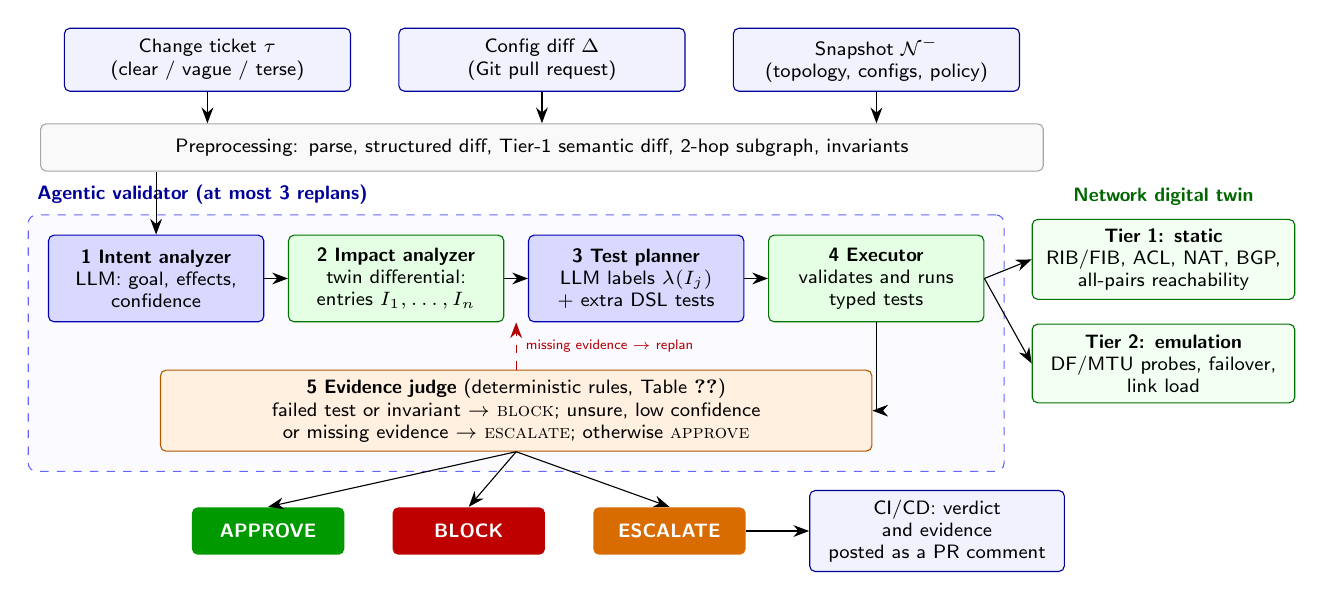
\begin{tikzpicture}[
  font=\sffamily\scriptsize, >={Stealth[length=2mm]}, node distance=4mm, execute at begin node={\hyphenpenalty=10000},
  inp/.style={draw=blue!60!black, fill=blue!5, rounded corners=2pt, align=center, minimum height=8mm, text width=34mm},
  llm/.style={draw=blue!70!black, fill=blue!15, rounded corners=2pt, align=center, minimum height=11mm, text width=25mm},
  det/.style={draw=green!45!black, fill=green!10, rounded corners=2pt, align=center, minimum height=11mm, text width=25mm},
  judge/.style={draw=orange!70!black, fill=orange!12, rounded corners=2pt, align=center, minimum height=10mm, text width=88mm},
  tier/.style={draw=green!45!black, fill=green!5, rounded corners=2pt, align=center, minimum height=10mm, text width=31mm},
  ver/.style={rounded corners=2pt, align=center, minimum height=6mm, text width=17mm, text=white, font=\sffamily\scriptsize\bfseries}]
\node[inp] (tkt) {Change ticket $\tau$\\(clear / vague / terse)};
\node[inp, right=6mm of tkt] (diff) {Config diff $\Delta$\\(Git pull request)};
\node[inp, right=6mm of diff] (snap) {Snapshot $\mathcal{N}^{-}$\\(topology, configs, policy)};
\node[draw=gray!70, fill=gray!5, rounded corners=2pt, align=center, text width=125mm, minimum height=6mm, below=4mm of diff] (pre) {Preprocessing: parse, structured diff, \mbox{Tier-1} semantic diff, 2-hop subgraph, invariants};
\node[llm, below=8mm of pre.south west, anchor=north west, xshift=1mm] (ia) {\textbf{1 Intent analyzer}\\LLM: goal, effects,\\confidence};
\node[det, right=3mm of ia] (imp) {\textbf{2 Impact analyzer}\\twin differential:\\entries $I_1,\dots,I_n$};
\node[llm, right=3mm of imp] (pl) {\textbf{3 Test planner}\\LLM labels $\lambda(I_j)$\\+ extra DSL tests};
\node[det, right=3mm of pl] (ex) {\textbf{4 Executor}\\validates and runs\\typed tests};
\node[judge, below=6mm of $(imp.south)!0.5!(pl.south)$] (jd) {\textbf{5 Evidence judge} (deterministic rules, Table~\ref{tab:judge})\\failed test or invariant $\to$ \textsc{block}; unsure, low confidence or missing evidence $\to$ \textsc{escalate}; otherwise \textsc{approve}};
\begin{scope}[on background layer]
\node[draw=blue!60, dashed, fill=blue!2, rounded corners=3pt, fit=(ia)(ex)(jd), inner sep=2.5mm, label={[font=\sffamily\scriptsize\bfseries, text=blue!60!black, anchor=south west]north west:Agentic validator (at most 3 replans)}] (box) {};
\end{scope}
\node[tier, below right=-2mm and 6mm of ex.north east, anchor=north west] (t1) {\textbf{Tier 1: static}\\RIB/FIB, ACL, NAT, BGP,\\all-pairs reachability};
\node[tier, below=3mm of t1] (t2) {\textbf{Tier 2: emulation}\\DF/MTU probes, failover,\\link load};
\node[font=\sffamily\scriptsize\bfseries, text=green!40!black, above=0.5mm of t1] {Network digital twin};
\node[ver, fill=green!60!black, below=7mm of jd.south west, anchor=north west, xshift=4mm] (A) {APPROVE};
\node[ver, fill=red!75!black, right=6mm of A] (B) {BLOCK};
\node[ver, fill=orange!85!black, right=6mm of B] (E) {ESCALATE};
\node[inp, text width=30mm, right=8mm of E] (ci) {CI/CD: verdict and evidence\\posted as a PR comment};
\draw[->] (tkt) -- (tkt|-pre.north);
\draw[->] (diff) -- (pre);
\draw[->] (snap) -- (snap|-pre.north);
\draw[->] (pre.south -| ia.north) -- (ia.north);
\draw[->] (ia) -- (imp); \draw[->] (imp) -- (pl); \draw[->] (pl) -- (ex);
\draw[->] (ex.east) -- (t1.west);
\draw[->] (ex.east) -- (t2.west);
\draw[->] (ex.south) |- (jd.east);
\draw[->, dashed, red!70!black] (jd.north) -- node[right, font=\sffamily\tiny, text=red!70!black]{missing evidence $\to$ replan} (jd.north|-pl.south);
\draw[->] (jd.south) -- (A.north);
\draw[->] (jd.south) -- (B.north);
\draw[->] (jd.south) -- (E.north);
\draw[->] (E.east) -- (ci.west);
\end{tikzpicture}
\caption{Architecture of NetVal. Blue boxes use an LLM; green boxes and the orange judge are deterministic code. The impact analyzer enumerates every behavioural difference of the change on the twin; the LLM only labels these differences against the ticket and proposes tests for promised effects. The judge, not the LLM, issues the verdict.}\label{fig:arch}
\end{figure*}

\subsection{Two-tier network digital twin}\label{sec:twin}

The twin answers two kinds of question about a snapshot, at two levels of fidelity.

\textbf{Tier 1 (static analysis)} computes the converged control plane $\Phi_1(\mathcal{N})$ in the style of Batfish~\cite{fogel2015batfish}: connected and static routes with next-hop resolution, OSPF~\cite{rfc2328} with adjacency compatibility checks (area, passive interfaces, subnet, hello and dead timers and MTU, where an MTU mismatch leaves the adjacency in the ExStart state), shortest paths with equal-cost multipath (ECMP), eBGP sessions with route-maps and prefix-lists, redistribution and administrative distance. Flows are traced symbolically through ingress and egress access control lists (ACLs, first match with implicit deny), NAT, VLAN and trunk attachment and every ECMP branch, producing a disposition such as \textsc{accepted}, \textsc{denied}, \textsc{no\_route}, \textsc{loop} or \textsc{no\_return}. Tier 1 is exhaustive over host pairs and services but has no notion of time, packet size or load.

\textbf{Tier 2 (emulation)} adds these three dimensions. A do-not-fragment probe of size $s$ is dropped at the first interface whose MTU is smaller than $s$. For a silent failure of link $e$, the traffic-loss time of a flow is
\begin{equation}
\begin{split}
T_{\mathrm{loss}}(e) &= T_{\mathrm{det}} + h\,T_{\mathrm{flood}} + T_{\mathrm{spf}} + T_{\mathrm{fib}},\\
T_{\mathrm{det}}&=\begin{cases}3\times 0.3\,\mathrm{s} & \text{with BFD~\cite{rfc5880}},\\ T_{\mathrm{dead}} & \text{otherwise},\end{cases}
\end{split}\label{eq:conv}
\end{equation}
where $h$ is the number of flooding hops, $T_{\mathrm{flood}}$ the per-hop flooding delay, $T_{\mathrm{spf}}$ the SPF throttle delay and $T_{\mathrm{fib}}$ the forwarding-table update time; a flow that loops or has no alternative path has $T_{\mathrm{loss}}=\infty$. The utilisation of link $e$ under the traffic matrix $D$ is $u_e=\sum_{d\in D} D_d\,\sigma_d(e)/\mathrm{cap}_e$, where $\sigma_d(e)$ is the share of demand $d$ that ECMP routes over $e$. Tier 2 answers only the concrete probes it is asked to send.

\subsection{Impact analyzer}\label{sec:impact}

The impact analyzer computes the differential behaviour of the change, $\mathcal{I}(c)=\Phi_1(\mathcal{N}^{+})\ominus\Phi_1(\mathcal{N}^{-})$, as a list of numbered entries $I_1,\dots,I_n$: changed flow dispositions per source, destination and service; routes added or removed per device; adjacencies and BGP sessions that changed state; changed forwarding paths; links that receive shifted demand under $D$; and Tier-2-relevant configuration objects (MTU, timer, BFD and SPF changes), which have no Tier-1 footprint but must be tested on Tier 2. This component is deterministic because the blast radius is computable exactly; asking an LLM to guess it would only add errors (Section~\ref{sec:ablation}).

\subsection{Intent analyzer and test planner}\label{sec:planner}

The \emph{intent analyzer} reads the ticket (and the diff only to resolve device names) and returns the goal, scope, expected effects, objects that must not change and a confidence $\gamma\in\{\text{high},\text{medium},\text{low}\}$ judged from the ticket text alone. Its rubric assigns \emph{low} when the ticket is only an identifier, in which case the analyzer must not infer a purpose from the diff, because the diff may contain the very mistake under test.

The \emph{test planner} receives the context package (ticket, intent analysis, structured diff, 2-hop topology subgraph, host list, invariants, impact entries and the DSL reference) and returns a labelling $\lambda:\mathcal{I}\rightarrow\{\text{intended},\text{unintended},\text{unsure}\}$ and a list $E$ of extra tests for effects the ticket promises but the impact list may not contain (for example, that a 9000-byte frame passes between two hosts). Each labelled entry is compiled deterministically into a test: an intended entry asserts the new behaviour, an unintended entry asserts that the behaviour is unchanged, and load, MTU and timer entries always become Tier-2 safety tests. The test plan is
\begin{equation}
\begin{split}
P(c) = \{\mathrm{compile}(I_j,\lambda(I_j)) &: \lambda(I_j)\neq\text{unsure}\}\\
&\cup\;E\;\cup\;V,
\end{split}\label{eq:plan}
\end{equation}
where $V$ is the set of invariant tests (no forwarding loops, management reachability, tenant isolation and no leak of internal prefixes), appended to every plan in the spirit of MeshAgent~\cite{zhou2025meshagent}.

Following LLNet~\cite{angi2025llnet}, the LLM never writes scripts. Tests are objects of a typed DSL (Table~\ref{tab:dsl}) that the executor validates before running; unknown types, unknown objects and missing fields are reported as invalid. The executor runs each test on the cheapest tier that can answer it.

\begin{table*}[t]
\caption{Typed test DSL. Tier indicates which twin tier can execute the test.}\label{tab:dsl}
\centering\footnotesize
\begin{tabular}{@{}lL{43mm}cL{50mm}@{}}
\toprule
Test & Fields & Tier & Meaning\\
\midrule
\texttt{reach} & src, dst, svc$|$*, expect allow/deny/unchanged & 1, 2 & flow disposition, including the return path\\
\texttt{path} & src, dst, via, expect & 1, 2 & all ECMP paths traverse a router\\
\texttt{route} & dev, prefix, expect present/absent/unchanged & 1, 2 & route in a device's RIB\\
\texttt{acl} & dev, acl, src, dst, svc, expect & 1 & formal ACL decision\\
\texttt{adj} & a, b, expect up/down/unchanged & 1, 2 & OSPF adjacency on a link\\
\texttt{like} & host, as & 1, 2 & a moved host has exactly the access of a reference host\\
\texttt{mtu} & src, dst, size, expect pass/fail & 2 & do-not-fragment probe\\
\texttt{conv} & a, b, max\_s & 2 & traffic-loss time after a silent link failure, Eq.~\eqref{eq:conv}\\
\texttt{load} & a, b, max\_pct & 2 & link utilisation under the traffic matrix\\
\texttt{inv} & no\_loops / mgmt\_reachable / isolation / no\_leak & 1 & network invariants (appended automatically)\\
\botrule
\end{tabular}
\end{table*}

\subsection{Evidence judge and bounded replanning}\label{sec:judge}

The judge applies the rules of Table~\ref{tab:judge} in order. Impact coverage is the share of impact entries (excluding pure path entries) for which at least one executed test produced evidence. A missing tier, an invalid test or an uncovered entry therefore never leads to approval: the planner is asked to repair the plan, and if evidence is still missing after three replans the change is escalated. Algorithm~\ref{alg:netval} summarises the complete procedure.

\begin{table}[t]
\caption{Deterministic evidence-judge rules, checked in order.}\label{tab:judge}
\centering\footnotesize
\begin{tabular}{@{}cL{42mm}L{20mm}@{}}
\toprule
Order & Condition & Verdict\\
\midrule
1 & Any executed test or invariant fails & \textsc{block}\\
2 & Any impact entry is labelled unsure & \textsc{escalate}\\
3 & Intent confidence $\gamma$ is low and the change alters behaviour & \textsc{escalate}\\
4 & Invalid tests, an impact entry without evidence, or no test confirms a promised effect & replan ($\le$3), then \textsc{escalate}\\
5 & Otherwise: all tests pass, 100\% impact coverage, no tool error & \textsc{approve}\\
\botrule
\end{tabular}
\end{table}

\begin{algorithm*}[t]
\caption{NetVal validation of one change}\label{alg:netval}
\footnotesize
\begin{algorithmic}[1]
\Require ticket $\tau$, diff $\Delta$, snapshot $\mathcal{N}^{-}$, invariants $V$, replan budget $R=3$
\State $\mathcal{N}^{+}\gets\mathcal{N}^{-}\oplus\Delta$; $X\gets\textsc{ContextPackage}(\tau,\Delta,\mathcal{N}^{-},k{=}2)$
\State $(\text{goal},\text{effects},\gamma)\gets\textsc{IntentAnalyzer}_{\mathrm{LLM}}(\tau,\Delta)$
\State $\mathcal{I}\gets\Phi_1(\mathcal{N}^{+})\ominus\Phi_1(\mathcal{N}^{-})\;\cup\;\textsc{Tier2Objects}(\Delta)$ \Comment{deterministic}
\State $\text{feedback}\gets\emptyset$
\For{$r=0$ \textbf{to} $R$}
  \State $(\lambda,E)\gets\textsc{Planner}_{\mathrm{LLM}}(X,\text{goal},\text{effects},\mathcal{I},\text{feedback})$
  \State $P\gets\{\textsc{Compile}(I_j,\lambda(I_j)) : \lambda(I_j)\neq\text{unsure}\}\cup E\cup V$
  \State $\text{res}\gets\textsc{Execute}(P,\mathcal{N}^{-},\mathcal{N}^{+})$ \Comment{cheapest tier per test}
  \If{any test in res fails} \Return \textsc{block} \EndIf
  \If{$\exists j:\lambda(I_j)=\text{unsure}$ \textbf{or} ($\gamma=\text{low}$ \textbf{and} $\mathcal{I}\neq\emptyset$)} \Return \textsc{escalate} \EndIf
  \State $\text{missing}\gets\textsc{Invalid}(\text{res})\cup\textsc{Uncovered}(\mathcal{I},\text{res})\cup\textsc{UnconfirmedEffects}(\text{effects},\text{res})$
  \If{$\text{missing}=\emptyset$} \Return \textsc{approve} \EndIf
  \State $\text{feedback}\gets\text{missing}$
\EndFor
\State \Return \textsc{escalate}
\end{algorithmic}
\end{algorithm*}

\subsection{Changes after Phase 2}\label{sec:changes}

The methodology was proposed in an earlier phase of this project. No written feedback was received on it, so Table~\ref{tab:changes} records every deviation of the implementation from the plan and its reason.

\begin{table*}[t]
\caption{Deviations of the implementation from the planned methodology.}\label{tab:changes}
\centering\footnotesize
\begin{tabular}{@{}L{34mm}L{42mm}L{42mm}@{}}
\toprule
Planned & Implemented & Reason and effect\\
\midrule
Tier 1 Batfish, Tier 2 containerlab with FRRouting & Python twin with the same two tiers, verified by 12 protocol-behaviour tests & No container runtime on the available machine; protocol fidelity is lower than real FRRouting\\
Measured tool time & Modelled CI time (Table~\ref{tab:cost}) plus measured LLM latency & The Python twin answers in milliseconds, which would make time comparisons meaningless\\
Labels checked by two annotators & Labels from an exhaustive oracle; variants that disagree with it discarded & Reproducible labels for 360 change--ticket pairs\\
Impact analyzer as an LLM agent & Deterministic Tier-1 differential & The blast radius is computable exactly\\
Planner writes the whole plan & Planner labels entries and adds extra tests; entries compiled to tests & Fewer output tokens and no hallucinated object names\\
-- & New DSL test \texttt{like}; host MTU in the context & Found during prompt tuning on the tuning split\\
Five repeats, local model on all runs & Three repeats (hosted); local model on a 32-case subset & API cost and local inference speed (2--4 tokens/s)\\
\botrule
\end{tabular}
\end{table*}

%=====================================================================
\section{Experimental setup}\label{sec:setup}
%=====================================================================

\subsection{Topologies}\label{sec:topologies}

Three networks were built (Figure~\ref{fig:topologies}). The \emph{campus} network has 10 devices, 14 hosts and 13 links, with OSPF, eBGP to an ISP, NAT, four user VLANs on three access switches and five ACLs. The \emph{data-centre} network is a leaf-spine fabric with 2 spines, 6 leaves acting as layer-3 gateways and 2 border routers peering with a WAN (12 devices, 11 hosts, 20 links, two tenants and jumbo-frame servers). The \emph{ISP} network is the 14-router NSFNET backbone from the Internet Topology Zoo~\cite{knight2011zoo} with three customers (one dual-homed), two upstream peers and management VLANs (20 devices, 9 hosts, 28 links). Configurations are text files in an IOS/FRRouting-like dialect, so every change is a real text diff. Each snapshot also contains the host inventory, the operator's intent policy (invariants and SLAs: failover within 3\,s and link utilisation below 90\%) and a traffic matrix.

\begin{figure*}[t]
\centering
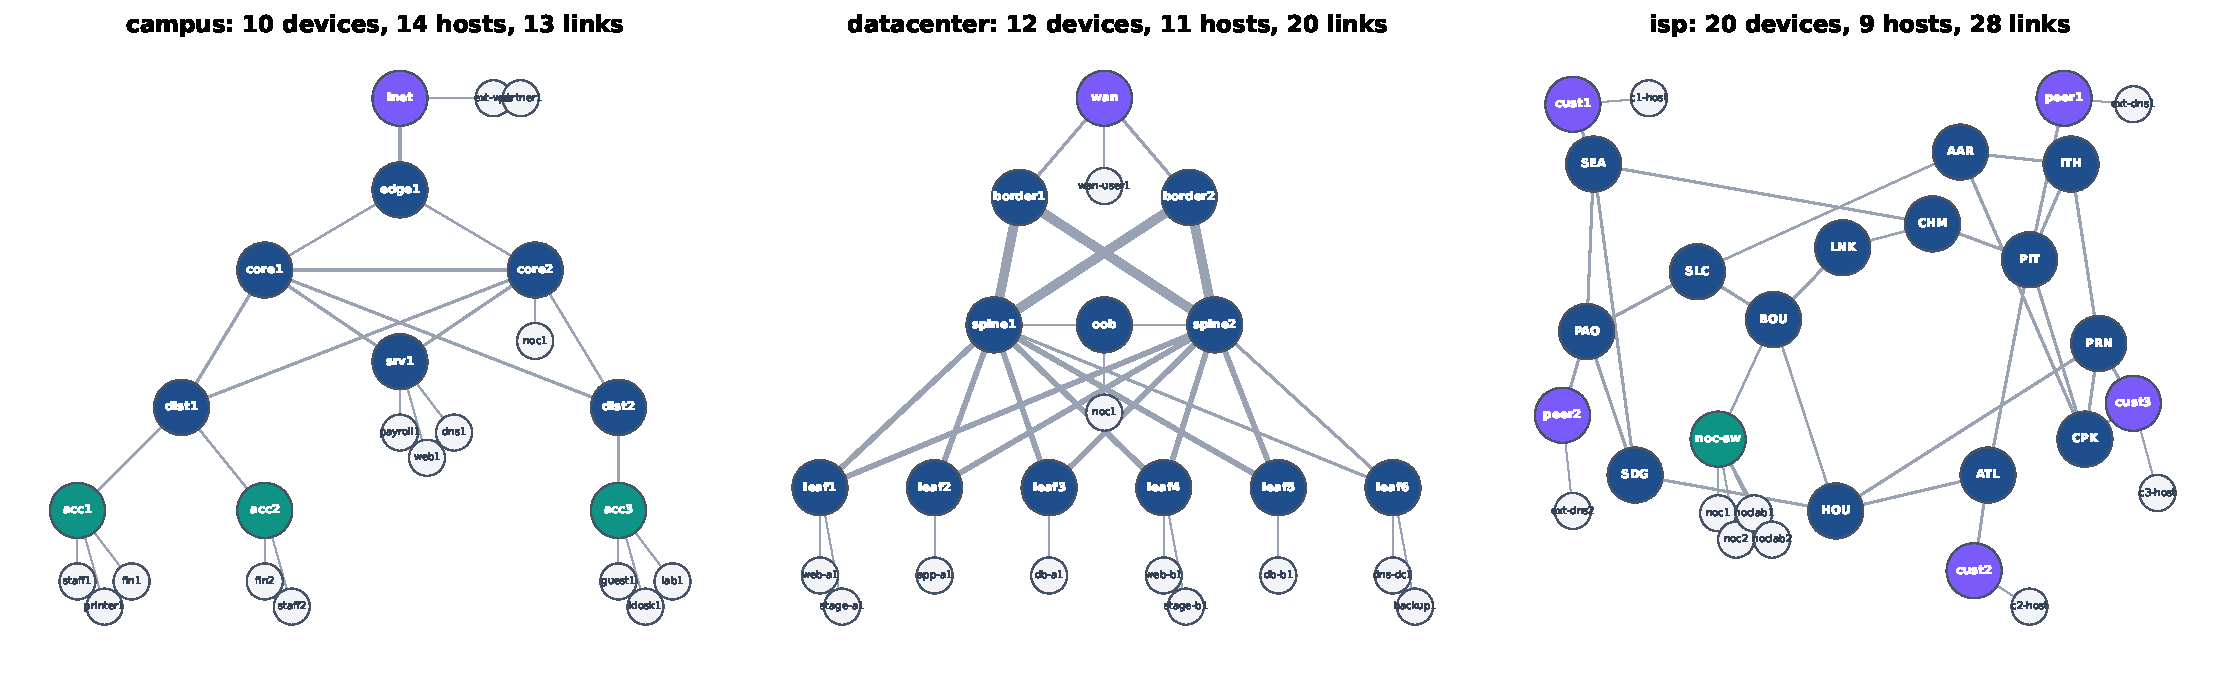
\includegraphics[width=0.92\textwidth]{figures/fig_topologies.pdf}
\caption{The three lab topologies (dark blue: routers; teal: layer-2 switches; purple: external autonomous systems; white: hosts). Line width is proportional to link capacity. Campus is used for prompt tuning only; data centre and ISP form the held-out test split.}\label{fig:topologies}
\end{figure*}

\subsection{Dataset}\label{sec:dataset}

\paragraph{Change cases.} A generator with 62 change templates produces realistic change requests in eight classes: ACL edits, static routes, OSPF cost and timer changes, BGP route-map and prefix-list changes, VLAN moves, MTU changes, interface maintenance (shutdown or drain) and NAT or redistribution. For most templates, a correct and a faulty implementation of the same ticket are generated; faults follow the families used by NetArena~\cite{zhou2026netarena} and CORNETTO~\cite{asadli2026cornetto}, such as wrong port, shadowed rule, over-broad rule, unresolvable next hop, one-sided OSPF cost, timer mismatch, removed BFD, MTU set on one end only, prefix-list typo, route-map leak, redistribution without a route-map, wrong VLAN identifier and shutdown of the wrong interface. Some templates are fault-only: the diff does exactly what the ticket asks, but the ticket itself is harmful (for example, draining a link that overloads the backup path). The dataset contains 120 changes (62 unsafe, 58 safe) and 28 distinct fault families (Figure~\ref{fig:dataset}).

\paragraph{Ticket versions.} Following Cleverest~\cite{liu2026cleverest}, every change has three tickets: \emph{clear} (devices, objects and expected effect), \emph{vague} (goal only) and \emph{terse} (identifier only). For template D-ACL-1 these are ``Staging needs database access: on leaf3 add `25 permit tcp 10.101.2.0/24 10.103.1.0/24 eq 5432' to ACL\_DBA\_OUT (before the final deny). Only stage-a1 $\rightarrow$ db-a1 on tcp/5432 should open.'', ``Let the tenant-A staging server talk to the tenant-A database.'' and ``fix ticket \#8768''. The faulty and correct implementations share the same tickets, so the only signal that separates them is network behaviour.

\paragraph{Ground truth.} An exhaustive oracle profiles $\mathcal{N}^{-}$ and $\mathcal{N}^{+}$ with both tiers: all host pairs under seven services, every route on every device, every adjacency, all four invariants, 1500-byte and jumbo probes between all host pairs, the failover time of every redundant link and the utilisation of every link. Each template carries a machine-readable intent specification of the flows, routes, adjacencies, paths, probes or drained links that the ticket requests. A change is labelled unsafe if an invariant breaks, the intended effect is not achieved, or anything else changes that the intent does not explain. Generated variants whose oracle label disagrees with the generator's intent are discarded.

\begin{figure*}[t]
\centering
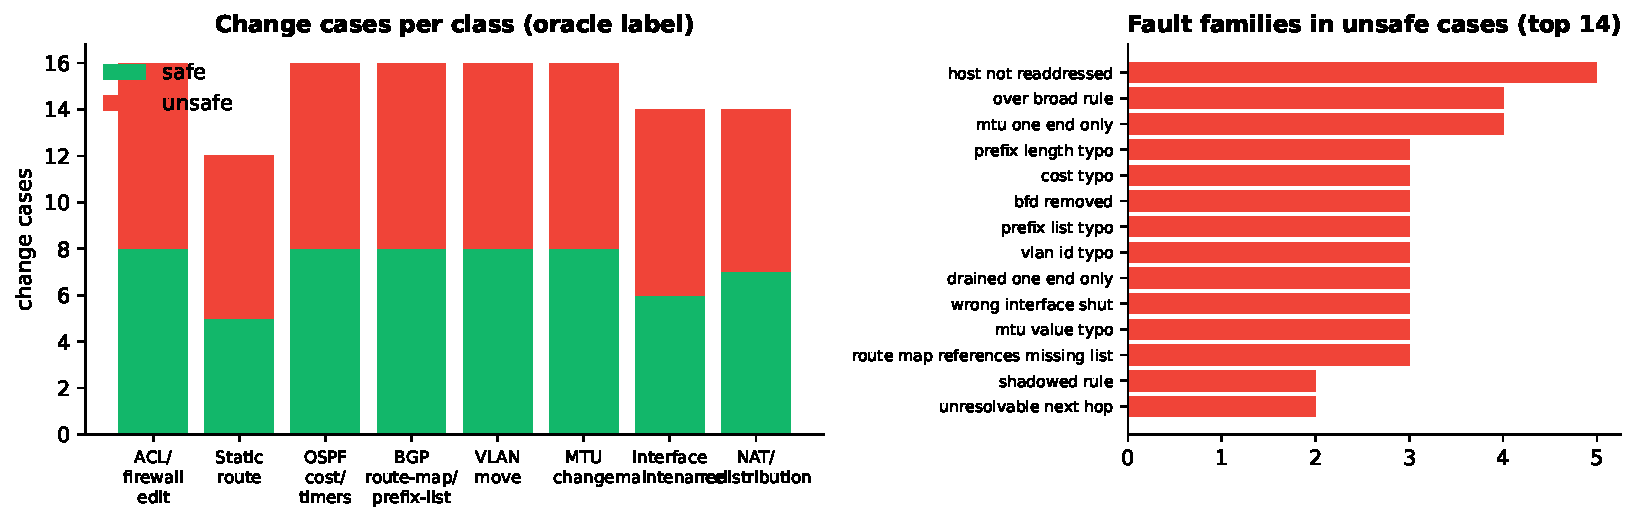
\includegraphics[width=0.72\textwidth]{figures/fig_dataset.pdf}
\caption{Dataset composition: safe and unsafe changes per change class (left) and the most frequent fault families among unsafe changes (right).}\label{fig:dataset}
\end{figure*}

\paragraph{Preprocessing and representation.} Every configuration is parsed into a vendor-neutral model, and the round trip $\mathrm{parse}(\mathrm{render}(x))=x$ is checked for every device. Two diffs are computed: a unified Git diff and a structured diff by device and configuration section. The Tier-1 differential is converted into numbered impact entries (Section~\ref{sec:impact}). The context package contains the ticket, the intent analysis, the structured diff, the 2-hop topology subgraph around the changed devices (devices, hosts and links with capacity), the host list with address, group and MTU, the invariants and SLAs, the impact entries and the DSL reference. The generated configurations contain no secrets.

\paragraph{Split.} To prevent prompt tuning on test data, the split is by topology: the campus network (33 changes, 99 change--ticket pairs, 27.5\%) is used only for prompt design, and the data-centre and ISP networks (87 changes: 45 unsafe and 42 safe, 261 change--ticket pairs) form the held-out test split. All results are reported on the test split.

\subsection{Baselines}\label{sec:baselines}

All methods run on identical changes and snapshots (paired design) and use the same twin and cost model.
\begin{itemize}
\item \textbf{B1 Fixed full suite.} Every change runs the same suite: all host pairs under seven services compared against the pre-change golden state, every route, every adjacency, the four invariants, 1500-byte probes between reachable hosts, failover of every redundant link and the utilisation of every link. Any deviation blocks. This represents current CI practice.
\item \textbf{B2 Rule-based selection.} If/else rules map the changed configuration section to a fixed test bundle around the changed device, plus the invariants. Any deviation blocks.
\item \textbf{B3 One-shot LLM.} The same hosted model receives the ticket, the unified diff and the device and host names, and writes a DSL plan in one call, without impact analysis, invariants, evidence rules or replanning. A failed test blocks; otherwise the change is approved. This re-implements the monolithic setting of CORNETTO~\cite{asadli2026cornetto}.
\item \textbf{B4 Static-only (Batfish-style).} No LLM and no emulation: Tier-1 invariants plus the full Tier-1 differential. A violated invariant blocks, any behavioural difference escalates and no difference approves. This represents a verifier-only gate.
\end{itemize}

\subsection{Metrics and statistical analysis}\label{sec:metrics}

The primary metrics are DR, FAR, FBR and AUTO (Eqs.~\eqref{eq:dr}--\eqref{eq:fbr}). Secondary metrics are the escalation rate and escalation precision (the share of escalations that are unsafe), the correct-verdict rate (unsafe blocked or safe approved), required-test coverage (the share of the expert-required tests stored with each template that the plan contains), the number of executed tests, CI time (Eq.~\eqref{eq:time}), LLM tokens and cost, and verdict consistency over repeats. Rates are reported with 95\% bootstrap confidence intervals~\cite{efron1979bootstrap} that resample whole changes (2{,}000 resamples, seed 0). Paired verdict outcomes are compared with the exact McNemar test~\cite{mcnemar1947}, test counts and times with the Wilcoxon signed-rank test~\cite{wilcoxon1945}, and $p$-values are corrected with the Holm procedure~\cite{holm1979}. Agreement across repeated runs is measured with Fleiss' $\kappa$~\cite{fleiss1971}.

\subsection{Implementation details}\label{sec:impl}

The prototype has about 6{,}600 lines of Python. The hosted LLM is Claude Sonnet~5.5 (\texttt{claude-sonnet-5-5}, Anthropic API) with effort ``medium''; the API does not accept a temperature setting for this configuration, so its default is used. The local LLM is Qwen2.5-7B-Instruct~\cite{qwen2025qwen25} (Q4\_K\_M quantisation) served by Ollama~0.40.16 with temperature 0.2, JSON output mode, a context of 6{,}144 tokens, and the repeat index as the seed. Other hyperparameters are a replan budget of $R=3$, an impact-coverage threshold of 100\% and a subgraph radius of $k=2$ hops. The dataset generator uses seed 7. Every LLM call is cached on disk, keyed by model, prompts and seed, so the full evaluation replays offline. The hosted agent ran three repeats on every test change and ticket version (783 runs); baselines and ablations ran once on each pair because they are deterministic or, for B3 and the ablations, because of API cost. The local model ran on a stratified subset of 32 test changes with clear tickets because inference on the available laptop was slow. Experiments ran on an Apple MacBook with an M4 processor (10 cores) and 16\,GB of unified memory under macOS~26.5, with Python~3.12.15, NumPy~2.5, SciPy~1.18, NetworkX~3.7, statsmodels~0.15, Matplotlib~3.11, Flask~3.1 and the Anthropic SDK~2.8. The total API cost of all experiments was US\$23.56. A GitHub Actions job (\texttt{ci/validate\_pr.py}) maps the verdict to exit codes 0, 1 and 2 (approve, block, escalate) and posts the evidence as a PR comment.

Because the twin is implemented in Python and answers in milliseconds, CI time is modelled with the costs of the real tools that the twin replaces (Table~\ref{tab:cost}). The same costs apply to every method.

\begin{table*}[t]
\caption{CI time-cost model applied identically to all methods.}\label{tab:cost}
\centering\footnotesize
\begin{tabular}{@{}lrL{52mm}@{}}
\toprule
Operation & Cost (s) & Basis\\
\midrule
Tier-1 snapshot initialisation, pre and post ($\kappa_1$) & 25 & Batfish snapshot initialisation, 10--20 devices\\
Tier-1 query ($\kappa(t)$; one all-pairs batch for B1/B2) & 1 & Batfish question latency\\
Tier-2 lab boot and convergence ($\kappa_2$) & 150 & containerlab with FRRouting, 10--20 nodes\\
Tier-2 probe (ping, traceroute, MTU) & 3 & per probe\\
Tier-2 failover experiment (\texttt{conv}) & 45 & fail link, reconverge, restore\\
Tier-2 load measurement (\texttt{load}) & 20 & one traffic run (all links at once for B1)\\
\botrule
\end{tabular}
\end{table*}

%=====================================================================
\section{Results and analysis}\label{sec:results}
%=====================================================================

\subsection{Main comparison}\label{sec:main}

Table~\ref{tab:main} and Figure~\ref{fig:main} report the results on the 87 test changes with clear tickets. The agent detected 97.8\% of unsafe changes, approved 2.2\% of them (one change) and blocked 4.8\% of safe changes, while auto-approving 92.9\% of safe changes. It is the only method that is good on both sides at once. B1 detected 80.0\% but blocked 61.9\% of safe changes, because every intended behaviour change is a deviation from the golden state; it also approved 20.0\% of unsafe changes, namely changes that do nothing or the wrong thing without breaking anything that held before (wrong port, one-sided cost, a link drained at one end only). A golden-state suite cannot know that the ticket asked for a new route or a new permit. B2 reduced the suite to 120 tests but missed faults whose effect appears away from the changed device (overloaded backup paths, leaks visible only at the peer), giving 40.0\% false approvals. B4 never blocked a safe change, but it is not a usable gate: it escalated 59.8\% of all changes and approved every unsafe change without a static footprint, that is, 40.0\% of unsafe changes.

B3 shows that the model alone is not the contribution. With the same model, it matched the agent's detection on clear tickets (97.8\%) but blocked 50.0\% of safe changes, because many of its own expectations were wrong; its plans covered only 30.5\% of the required tests against 94.3\% for the agent. The difference becomes visible with poorer tickets (Section~\ref{sec:intent}).

\begin{table*}[t]
\caption{Results on the test split (87 changes, clear tickets, first run of each method; 95\% bootstrap confidence intervals in brackets). DR: detection rate; FAR: false-approval rate; FBR: false-block rate; Esc.: escalation rate; AUTO: safe auto-approval; Cov.: required-test coverage; Tests: mean tests executed; Time: mean modelled CI time.}\label{tab:main}
\centering\footnotesize
\begin{tabular}{@{}lcccccccr@{}}
\toprule
Method & DR (\%) & FAR (\%) & FBR (\%) & Esc. & AUTO & Cov. & Tests & Time (min)\\
\midrule
B1 Fixed full suite & 80.0 [68,91] & 20.0 [9,32] & 61.9 [49,76] & 0.0 & 38.1 & 90.2 & 1559.4 & 20.5\\
B2 Rule-based & 60.0 [46,74] & 40.0 [26,54] & 54.8 [40,69] & 0.0 & 45.2 & 84.4 & 119.7 & 1.8\\
B4 Static only & 60.0 [45,73] & 40.0 [27,55] & 0.0 [0,0] & 59.8 & 38.1 & 64.0 & 6.4 & 0.8\\
B3 One-shot LLM & 97.8 [93,100] & 2.2 [0,7] & 50.0 [34,65] & 0.0 & 50.0 & 30.5 & 28.4 & 3.7\\
\textbf{NetVal (hosted)} & \textbf{97.8} [93,100] & \textbf{2.2} [0,7] & 4.8 [0,12] & 2.3 & \textbf{92.9} & \textbf{94.3} & 12.2 & 2.4\\
\botrule
\end{tabular}
\end{table*}

\begin{figure*}[t]
\centering
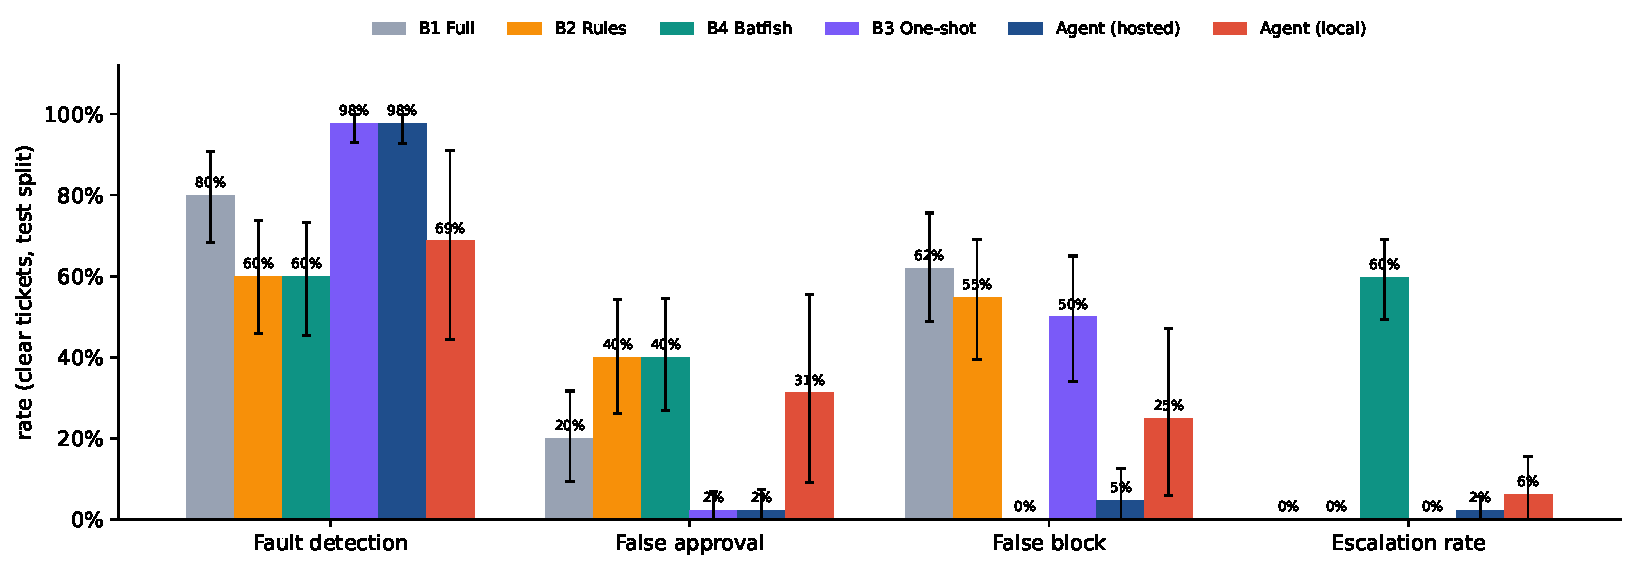
\includegraphics[width=0.8\textwidth]{figures/fig_main_rates.pdf}
\caption{Detection, false-approval, false-block and escalation rates per method on clear tickets, with 95\% bootstrap intervals. The local agent is evaluated on its 32-change subset.}\label{fig:main}
\end{figure*}

\paragraph{Variability over repeated runs.} Table~\ref{tab:main} uses the first run of each method so that all methods are compared on one run. Over the three repeats of the hosted agent, the clear-ticket rates were DR $96.3\pm1.3$\%, FAR $3.7\pm1.3$\%, FBR $3.2\pm1.4$\%, escalation $1.1\pm1.1$\%, AUTO $95.2\pm2.4$\%, $12.3\pm0.2$ tests and $146\pm3$\,s (mean $\pm$ standard deviation). Fleiss' $\kappa$ over the repeats is 0.92, and 92.0\% of change--ticket pairs received the same verdict in all three runs. The deterministic judge on top of the LLM keeps the gate stable.

\subsection{Efficiency}\label{sec:efficiency}

Figure~\ref{fig:efficiency} relates detection to cost. The agent ran 12.2 tests per change on average, 128 times fewer than B1, and needed 2.4 modelled minutes instead of 20.5 (an 8.6-fold reduction), including 6.3\,s of LLM time. Most of the remaining time is the Tier-2 boot, which is paid only when a Tier-2 test is required; the median CI time was 56\,s. The agent is not the fastest method: B2 (1.8\,min) and B4 (0.8\,min) are cheaper because they never boot the emulation tier or because B4 never decides, but both approve 40\% of unsafe changes. The hosted model consumed 4{,}859 tokens and US\$0.015 per change, about US\$15 per 1{,}000 PRs.

\begin{figure*}[t]
\centering
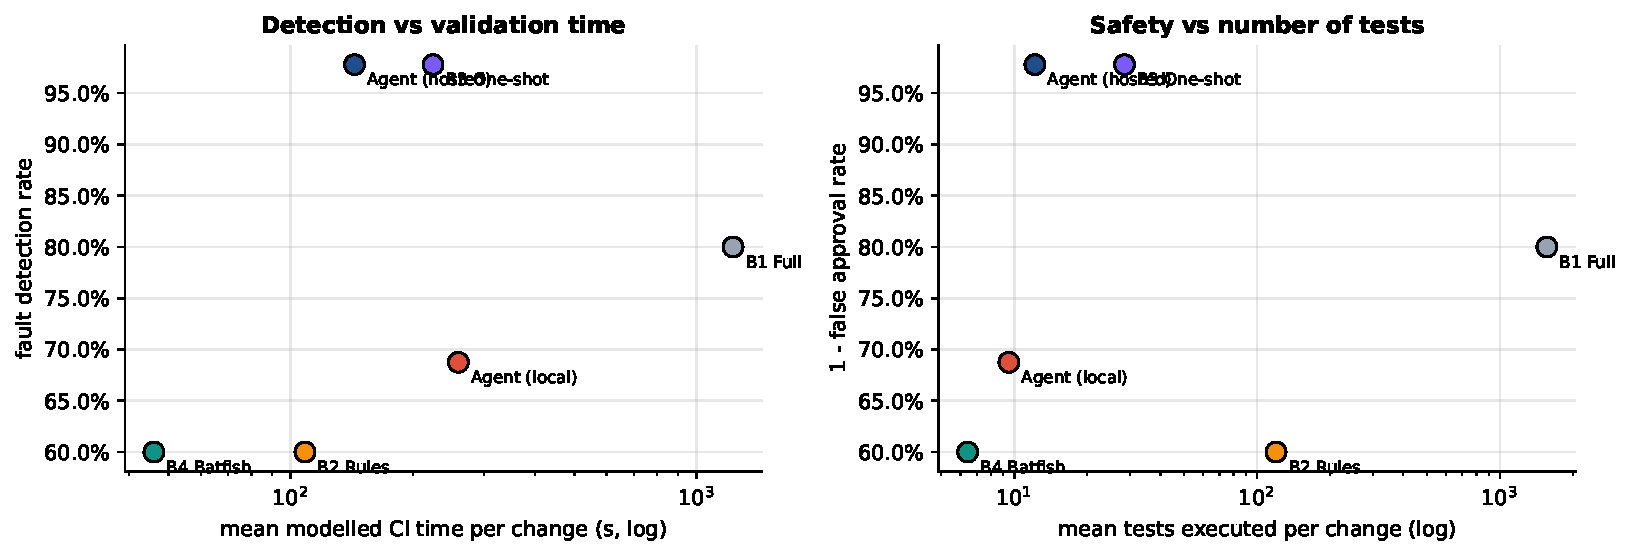
\includegraphics[width=0.75\textwidth]{figures/fig_time_vs_detection.pdf}
\caption{Detection against modelled CI time per change (left) and safety ($1-\mathrm{FAR}$) against the number of executed tests (right), clear tickets. The upper-left corner is better.}\label{fig:efficiency}
\end{figure*}

\subsection{Effect of ticket quality}\label{sec:intent}

Figure~\ref{fig:intent} varies the ticket. With vague tickets, the agent's detection fell from 97.8\% to 91.1\% and its false-approval rate rose to 8.9\% (mean over repeats $12.6\pm4.6$\%): given only a goal, the planner sometimes accepted a side effect as part of that goal. With terse tickets, the agent behaved as designed. The intent analyzer reported low confidence, the planner labelled entries unsure, and the gate escalated 86.2\% of changes and approved none; unsafe changes whose failures are independent of intent (invariants, MTU, load and failover) were still blocked, so the false-approval rate was 0.0\% in all three repeats. B3, which cannot abstain, approved 11.1\% of unsafe changes with vague tickets and 22.2\% with terse tickets. Ticket quality therefore determines how much of the validation can be automated, while the gate remains safe.

\begin{figure*}[t]
\centering
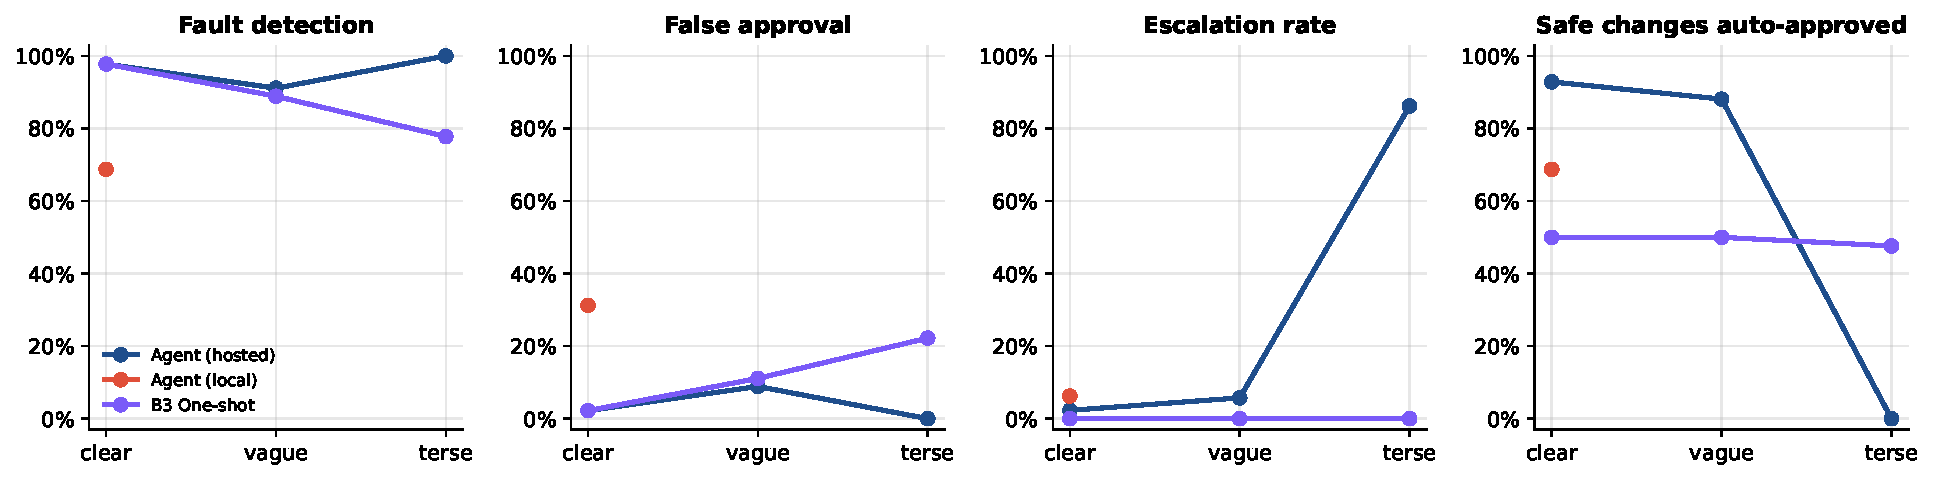
\includegraphics[width=0.9\textwidth]{figures/fig_intent_quality.pdf}
\caption{Effect of ticket quality (clear, vague, terse) on the LLM-based methods. The local agent was evaluated on clear tickets only.}\label{fig:intent}
\end{figure*}

\subsection{Twin tiers and change classes}\label{sec:tiers}

Figure~\ref{fig:tiers} shows which tier produced the blocking evidence for each unsafe change the agent blocked on clear tickets: Tier 1 for 34 changes and Tier 2 for 9. Independently of the agent, 18 unsafe changes leave no static trace at all (B4 approves them); they include MTU value typos, removed BFD, SPF delay typos, overloaded backup paths and static routes that loop only after a failure. These changes justify the emulation tier. Broken down by change class, B4's false approvals concentrate in OSPF, ACL, static-route, MTU and maintenance changes, and B2's misses are spread over five classes. The agent's four non-correct verdicts on clear tickets occurred in OSPF (2), static route (1) and VLAN move (1), and its only false approval is a static route (Section~\ref{sec:failures}).

\begin{figure}[t]
\centering
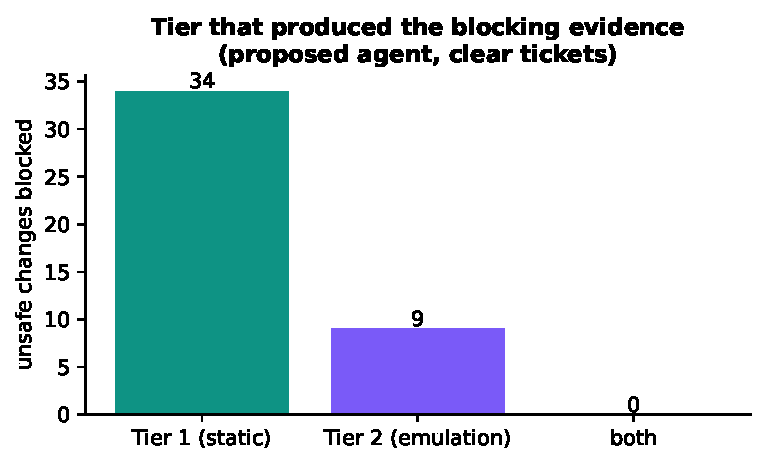
\includegraphics[width=0.8\columnwidth]{figures/fig_tiers.pdf}
\caption{Twin tier that produced the blocking evidence for each unsafe change blocked by the agent (clear tickets). Tier 1 handled most faults cheaply; Tier 2 was decisive for faults that involve packet size, timers, load or failure.}\label{fig:tiers}
\end{figure}

\subsection{Statistical significance}\label{sec:stats}

Table~\ref{tab:stats} reports paired tests over all three ticket versions (261 pairs). The agent detected significantly more unsafe changes than B1, B2 and B4 and blocked significantly fewer safe changes than B1, B2 and B3 (Holm-corrected $p<0.01$). It ran significantly fewer tests than B1, B2 and B3 and was faster than B1 and B3, but slower than B2 and B4. Against B3, the difference in detection was not significant ($p=0.134$), and against B4 the difference in false blocks was not significant ($p=0.156$). The local-model comparison has only 32 pairs and is not significant.

\begin{table*}[t]
\caption{Paired comparison of the hosted agent with each method over all ticket versions. For verdict outcomes, the counts give pairs where only the agent (A) or only the other method (O) has the property, with exact McNemar tests; tests and time give the median paired difference (agent minus other) with Wilcoxon signed-rank tests. All $p$-values are Holm-corrected.}\label{tab:stats}
\centering\footnotesize
\begin{tabular}{@{}lrllll@{}}
\toprule
Other method & Pairs & Detected (A/O) & False block (A/O) & $\Delta$Tests & $\Delta$Time (s)\\
\midrule
B1 Fixed full suite & 261 & 27/5, $p=0.001$ & 4/76, $p<0.001$ & $-1446$, $p<0.001$ & $-1052$, $p<0.001$\\
B2 Rule-based & 261 & 51/2, $p<0.001$ & 4/67, $p<0.001$ & $-17$, $p<0.001$ & $+8$, $p<0.001$\\
B4 Static only & 261 & 51/2, $p<0.001$ & 6/0, $p=0.156$ & $+2$, $p<0.001$ & $+5$, $p<0.001$\\
B3 One-shot LLM & 261 & 15/4, $p=0.134$ & 3/61, $p<0.001$ & $-17$, $p<0.001$ & $-26$, $p<0.001$\\
Agent, local 7B & 32 & 5/1, $p=0.656$ & 0/4, $p=0.500$ & $+3$, $p<0.001$ & $-99$, $p<0.001$\\
\botrule
\end{tabular}
\end{table*}

%=====================================================================
\section{Comparison with base papers and the state of the art}\label{sec:comparison}
%=====================================================================

\subsection{Base papers}\label{sec:base}

The work builds on five base papers. Aether~\cite{auge2026aether}, Khaldi et al.~\cite{khaldi2026agentic} and Nam et al.~\cite{nam2026vnf} defined the problem in the first phase of this project; CORNETTO~\cite{asadli2026cornetto} and Cleverest~\cite{liu2026cleverest} shaped the experimental design (one-shot baseline, verifier grounding, regression as a safety metric and ticket-quality variation). Table~\ref{tab:basepapers} summarises them.

\begin{table*}[t]
\caption{Summary of the base papers.}\label{tab:basepapers}
\centering\scriptsize
\begin{tabular}{@{}L{17mm}L{17mm}L{19mm}L{19mm}L{14mm}L{19mm}L{20mm}@{}}
\toprule
Paper & Problem & Method & Dataset & Metrics & Reported results & Key limitations\\
\midrule
Aug\'e et al.\ (2026), Aether~\cite{auge2026aether} & Validate network changes before deployment & Five GPT-4o agents; Batfish, NS-3, RouteNet via MCP; knowledge graph & 8 synthetic change scenarios; 2 ISP incidents; 25-router lab & Detection, precision, test coverage, time & 94\% faulty-change detection; 6--7\,min per change & No fixed-suite baseline; one model; ticket quality not varied\\
Khaldi et al.\ (2026)~\cite{khaldi2026agentic} & Design, test and operate digital twin networks & Multi-agent closed loop with versioned memory; several LLMs & Emulated 6G core; MEC and slicing use cases & Success, iterations, time & Up to 100\% success; loop adds 16.7--80\pp & Builds or operates the twin; does not judge PRs\\
Nam et al.\ (2026)~\cite{nam2026vnf} & Deploy VNFs from procedures & Nine LLMs, RAG, multi-agent debate, Kubernetes twin & 60 VNF procedures (Korean, English) & Deployment success, retries, time & 10\% zero-shot to 70--80\% with the agent & Checks deployment success, not policy safety\\
Asadli et al.\ (2026), CORNETTO~\cite{asadli2026cornetto} & Repair broken router configurations & ReAct agent with Batfish verifier vs one-shot prompting & 231 scenarios, Topology Zoo, up to 754 nodes, 27 fault types & Fix score, regression rate, cost & +12\% fix and +17\% safety over one-shot; regressions 34.2\% to $<$6\% & Static checks only; no human gate; 4--5$\times$ cost\\
Liu et al.\ (2026), Cleverest~\cite{liu2026cleverest} & Regression tests for software commits & GPT-4o with commit message and diff, execution feedback (5 rounds) & 72 commits from 8 C programs & Bugs found, time & 20 bugs with intent vs 4 without, in $<$2\,min & Software only; no blast radius; cost of unnecessary tests not measured\\
\botrule
\end{tabular}
\end{table*}

\subsection{Quantitative comparison}\label{sec:quant}

The base papers do not release their change sets or twins, so their numbers cannot be reproduced on the dataset of this study. Table~\ref{tab:quant} therefore combines two kinds of entries: the published headline results of the base papers (marked with an asterisk, on their own data and settings) and re-implementations of their method families on the dataset of this study, with the same twin, metrics and split. B3 re-implements the monolithic one-shot setting that CORNETTO uses as its reference, and B4 re-implements a verifier-only gate in the style of the Batfish analyses used by CORNETTO and Clarify. The conceptual Aether pipeline (agentic planning grounded in a twin) corresponds to NetVal without the deterministic impact analyzer, which is reported as an ablation (Section~\ref{sec:ablation}).

\begin{table*}[t]
\caption{Quantitative comparison. Rows marked $^{*}$ are values reported in the original papers on their own data and are not directly comparable; other rows were run on the test split of this study (87 changes, clear tickets unless stated).}\label{tab:quant}
\centering\footnotesize
\begin{tabular}{@{}L{60mm}cccc@{}}
\toprule
Method (source) & DR (\%) & FAR (\%) & FBR (\%) & Time/change\\
\midrule
Aether~\cite{auge2026aether}$^{*}$ (8 scenarios, wall-clock time) & 94 & n/r & n/r & 6--7\,min\\
CORNETTO agent~\cite{asadli2026cornetto}$^{*}$ (repair; regression rate) & n/a & $<$6$^{\dagger}$ & n/a & n/r\\
CORNETTO one-shot~\cite{asadli2026cornetto}$^{*}$ (repair; regression rate) & n/a & up to 34.2$^{\dagger}$ & n/a & n/r\\
\midrule
One-shot LLM, CORNETTO setting (B3, re-implemented) & 97.8 & 2.2 & 50.0 & 3.7\,min\\
\quad same, terse tickets & 77.8 & 22.2 & 52.4 & 3.3\,min\\
Verifier-only gate (B4, re-implemented) & 60.0 & 40.0 & 0.0 & 0.8\,min\\
Agent without impact analyzer (Aether-like planning; ablation) & 95.6 & 4.4 & 47.6 & 6.0\,min\\
Fixed full suite (B1, industry practice) & 80.0 & 20.0 & 61.9 & 20.5\,min\\
\textbf{NetVal} & \textbf{97.8} & \textbf{2.2} & \textbf{4.8} & 2.4\,min\\
\quad same, terse tickets & 100.0 & 0.0 & 0.0 & 2.0\,min\\
\botrule
\end{tabular}
\footnotetext{n/r: not reported; n/a: not applicable to the task. $^{\dagger}$Regression rate of repaired configurations, the closest analogue of false approval.}
\end{table*}

\subsection{Methodological comparison}\label{sec:methodcomp}

NetVal differs from the base papers in three design decisions. First, the blast radius is computed by the twin and not by the LLM. Aether asks agents to plan tests from the change and a knowledge graph; NetVal gives the planner an exhaustive list of what actually changed, so the LLM only decides which differences the ticket explains. This addresses the main failure mode of one-shot planning observed in B3, which guessed expectations for behaviour the ticket never mentioned. Second, the verdict is computed by deterministic rules with an explicit escalation path. CORNETTO reports no human gate for risky edits, and Aether returns a test outcome; NetVal escalates when the ticket is ambiguous, confidence is low or evidence is missing, which is the abstention principle of MeshAgent applied to a CI/CD verdict. Third, NetVal uses two twin tiers and records which tier produced each piece of evidence, addressing CORNETTO's limitation that static verification cannot see transient and performance faults. Unlike Khaldi et al.\ and Nam et al., the twin is used as a test bench for someone else's change rather than as the system being configured.

\subsection{Improvement analysis}\label{sec:improvement}

Relative to the fixed full suite (B1), NetVal improves detection by $+17.8$\pp (from 80.0\% to 97.8\%, a relative gain of 22.2\%), reduces false approvals by $17.8$\pp (from 20.0\% to 2.2\%, $-88.9$\% relative) and false blocks by $57.1$\pp (from 61.9\% to 4.8\%), with 99.2\% fewer tests and 88.3\% less CI time. The gain comes from intent: B1 cannot tell an intended difference from a regression and cannot test an effect that the ticket requests. Relative to the one-shot LLM (B3), detection on clear tickets is unchanged, but false blocks fall by $45.2$\pp (from 50.0\% to 4.8\%), required-test coverage rises from 30.5\% to 94.3\%, and on terse tickets false approvals fall from 22.2\% to 0.0\%. These gains come from the impact analyzer and the escalation rules. Relative to the verifier-only gate (B4), detection rises by $+37.8$\pp (from 60.0\% to 97.8\%) and false approvals fall from 40.0\% to 2.2\%, because Tier 2 and the intent labels give B4's escalations and silent approvals a decision. Against Aether's published 94\% detection, NetVal's 97.8\% is $+3.8$\pp higher, but the datasets, twins and time measurements differ, so this difference is indicative only.

\subsection{Fairness and limitations of the comparison}\label{sec:fairness}

Several factors limit the comparison. The base papers use different networks, change sets and tools, and none of their datasets are available, so their numbers are quoted rather than reproduced. Aether reports measured wall-clock time on real tools, whereas the times in this study are modelled with tool costs (Table~\ref{tab:cost}). CORNETTO measures regressions of repaired configurations, which is related to but not identical with approving an unsafe change. All methods in this study share the same twin and oracle, so a twin modelling error would affect both the methods and the labels. Finally, NetVal does not outperform every baseline on every metric: B4 has fewer false blocks (0.0\% vs 4.8\%, not significant), B2 and B4 are faster, B4 runs fewer tests, and B1 catches the static-route failover loop that NetVal misses (Section~\ref{sec:failures}).

%=====================================================================
\section{Ablation study}\label{sec:ablation}
%=====================================================================

Each component was removed or replaced in turn, and the test split was re-run with clear tickets. The tier ablations re-execute the same plans with one tier disabled, which isolates the twin from the LLM. Table~\ref{tab:ablation} and Figure~\ref{fig:ablation} report the results.

\begin{table*}[t]
\caption{Ablation results (test split, clear tickets unless stated; differences from the full agent in percentage points in parentheses).}\label{tab:ablation}
\centering\footnotesize
\begin{tabular}{@{}lcccccrr@{}}
\toprule
Variant & DR (\%) & FAR (\%) & FBR (\%) & Esc. (\%) & AUTO (\%) & Tests & Time (min)\\
\midrule
Full agent & 97.8 & 2.2 & 4.8 & 2.3 & 92.9 & 12.2 & 2.4\\
$-$ impact analyzer & 95.6 ($-2.2$) & 4.4 ($+2.2$) & 47.6 ($+42.8$) & 3.4 & 47.6 ($-45.3$) & 37.0 & 6.0\\
$-$ feedback loop & 97.8 (0.0) & 2.2 (0.0) & 4.8 (0.0) & 2.3 & 92.9 (0.0) & 12.2 & 2.4\\
$-$ invariant guard & 95.6 ($-2.2$) & 4.4 ($+2.2$) & 2.4 ($-2.4$) & 1.1 & 95.2 ($+2.3$) & 8.6 & 2.3\\
Tier 1 only (static) & 97.8 (0.0) & 2.2 (0.0) & 7.1 ($+2.3$) & 28.7 & 57.1 ($-35.8$) & 12.2 & 0.9\\
Tier 2 only (emulation) & 97.8 (0.0) & 2.2 (0.0) & 4.8 (0.0) & 2.3 & 92.9 (0.0) & 12.2 & 4.8\\
Vague tickets & 91.1 ($-6.7$) & 8.9 ($+6.7$) & 9.5 ($+4.7$) & 5.7 & 88.1 ($-4.8$) & 9.8 & 2.2\\
Terse tickets & 100.0 ($+2.2$) & 0.0 ($-2.2$) & 0.0 ($-4.8$) & 86.2 & 0.0 ($-92.9$) & 5.6 & 2.0\\
Local 7B model (32 changes) & 68.8 & 31.2 & 25.0 & 6.2 & 68.8 & 9.5 & 4.3\\
\botrule
\end{tabular}
\end{table*}

\begin{figure*}[t]
\centering
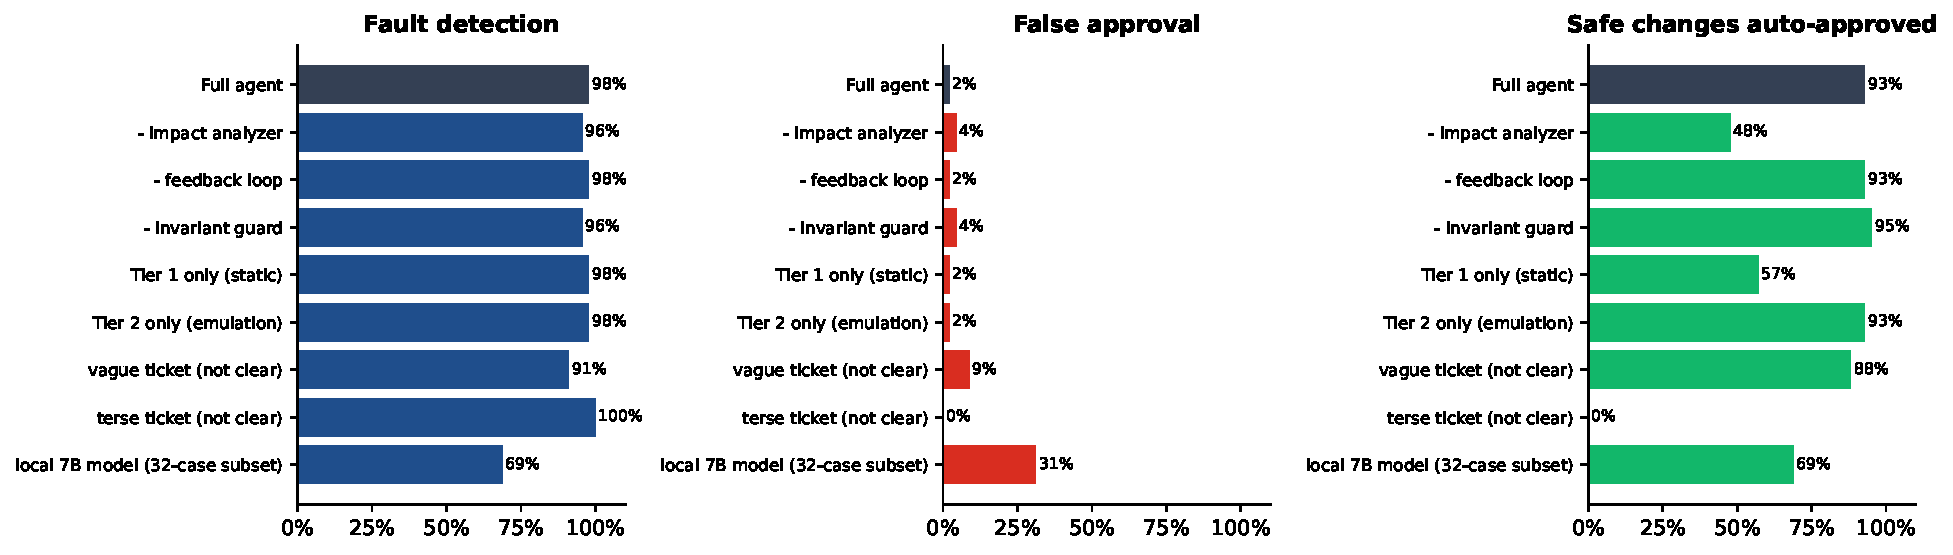
\includegraphics[width=0.88\textwidth]{figures/fig_ablation.pdf}
\caption{Ablation results: detection, false approval and safe auto-approval per variant.}\label{fig:ablation}
\end{figure*}

\paragraph{Impact analyzer.} Without the twin-computed blast radius, the planner must infer from the ticket and the raw diff what could be affected. It wrote 37 tests instead of 12, false approvals doubled to 4.4\%, and false blocks rose from 4.8\% to 47.6\% because the planner asserted ``unchanged'' on behaviour that the change legitimately alters or guessed wrong expectations. Safe auto-approval halved and CI time grew to 6.0 minutes. This is the most important component.

\paragraph{Feedback loop.} Removing replanning changed nothing, because in all 261 runs of the full hosted agent the first plan was already complete (zero replans). The loop is used when plans are incomplete: it fired in 13.8\% of runs without the impact analyzer and in 80.5\% of runs with Tier 1 only, where it converted missing evidence into escalations. On this dataset it is a safety valve rather than a contributor to accuracy.

\paragraph{Invariant guard.} Removing the automatically appended invariant tests (and the invariant text in the prompt) reduced detection to 95.6\% and doubled false approvals to 4.4\%, while slightly reducing false blocks. Most invariant violations also appear as unintended impact entries, so the guard acts as a safety net for entries that the LLM mislabels; required-test coverage fell from 94.3\% to 30.6\% because the expert test lists include the invariants.

\paragraph{Twin tiers.} With Tier 1 only, Tier-2 tests are skipped, so MTU, timer and load entries remain without evidence and the judge escalates instead of approving. False approvals stayed at 2.2\%, but escalations rose from 2.3\% to 28.7\% and safe auto-approval fell from 92.9\% to 57.1\%, while CI time fell to 0.9 minutes. The evidence rule therefore turns a missing tier into human work rather than risk. With Tier 2 only, verdicts were unchanged on this dataset, but every change paid the emulation boot (4.8 minutes instead of 2.4), formal ACL questions could not be answered and wildcard services were only sampled. Both tiers are needed: Tier 1 for exhaustive and cheap checks, and Tier 2 for evidence that static analysis cannot provide.

\paragraph{Model size.} On a stratified subset of 32 test changes with clear tickets, the local Qwen2.5-7B agent detected 68.8\% of unsafe changes with 31.2\% false approvals and 25.0\% false blocks, against 93.8\%, 6.2\% and 0.0\% for the hosted model on the same changes, and it needed about 120\,s of LLM time per change on the laptop (hosted: 6\,s). The deterministic components do not compensate for a weak planner: the 7B model often failed to test effects that the ticket promises (a route that should appear, a link that should be drained), so changes that silently do nothing were approved.

%=====================================================================
\section{Discussion}\label{sec:discussion}
%=====================================================================

\subsection{Why the method works}\label{sec:why}

The results support a division of labour between the LLM and deterministic code. Enumerating the blast radius is a computation, and the twin performs it exactly; deciding whether a difference is what the ticket asked for is a judgement about language, and the LLM performs it well when the ticket is clear. Because each LLM decision is a label on a concrete, twin-computed difference, a wrong label is usually caught by a failing test, an uncovered entry or an invariant. A false approval requires the LLM to label a harmful side effect as intended or to omit a test for a promised effect, and the evidence rules make the second case escalate whenever the effect is stated in the ticket. The same structure explains the behaviour on terse tickets: without intent, the LLM labels entries unsure, and the gate degrades to human review instead of guessing.

\subsection{Practical implications}\label{sec:implications}

Four recommendations follow for operators. Auto-approve only when no test fails, impact coverage is 100\%, intent confidence is high or medium and no entry is unsure. Always run Tier 2 when the impact includes MTU, timer, BFD, SPF or load-shift entries, or when a static route is added; the last rule would have removed the only clear-ticket false approval. Treat identifier-only tickets as ``escalate unless nothing behavioural changed'' and ask authors for one sentence of intent, which on this dataset moves most safe changes from human review to automatic approval. Keep a nightly full-suite run as a backstop, so that the fixed suite no longer blocks delivery but still catches failure-only risks. With a 7B local model, the gate should run in block-or-escalate mode only until a stronger local model is validated.

\subsection{Failure analysis}\label{sec:failures}

All 55 non-automated or wrong verdicts of the agent on the test split (out of 261 change--ticket pairs in the first run) were classified (Figure~\ref{fig:failures}). Forty-four were intended escalations on ambiguous tickets (42 terse, one vague and one clear). Six were bad tests, in which an extra test encoded a wrong expectation, such as a path through the wrong router. Three were missed dependencies, in which a fault appears only under failure and no impact entry prompted a failover test. Two were intent misreadings, in which the planner accepted an unintended behaviour change as part of the goal.

\begin{figure*}[t]
\centering
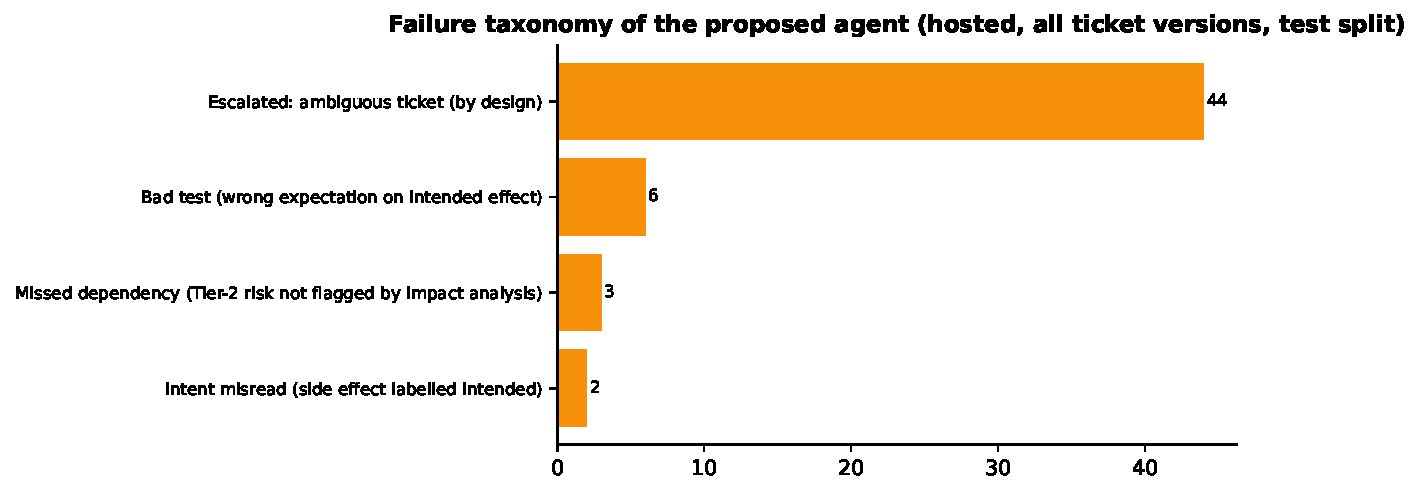
\includegraphics[width=0.62\textwidth]{figures/fig_failures.pdf}
\caption{Failure taxonomy of the hosted agent over all ticket versions on the test split.}\label{fig:failures}
\end{figure*}

\paragraph{Missed dependency (D-STA-1-F, false approval).} The ticket pins traffic from leaf1 towards app-a1 onto spine1 with a static route. The diff does exactly that, Tier 1 shows only path changes, which the planner correctly labels intended, and all 14 tests pass. When the leaf2--spine1 link fails silently, however, spine1 reroutes through other leaves while leaf1 keeps forcing traffic to spine1, creating a micro-loop and an unbounded outage between web-a1 and app-a1. Only a failover test reveals this, and B1 blocks the change because it tests failover on every link.

\paragraph{Intent misread with a vague ticket (D-ACL-2-F).} The clear ticket asks to deny tcp/443 from staging to the application subnet, but the faulty diff denies all IP traffic. With the clear ticket, the agent labels the extra denied services unintended and blocks. With the vague ticket (``Stop staging from hitting the production app''), blocking everything is a reasonable reading, so the planner labels it intended and approves: this is the ambiguity problem described by Clarify~\cite{mondal2025clarify}.

\paragraph{Correct escalation (I-BGP-1-S, terse ticket).} The ticket reads ``implements CHG-9791''. The intent analyzer reports low confidence, the impact analyzer finds a new route 172.16.11.0/24, the planner labels it unsure, and the gate escalates. B1 and B2 block this safe change, and B4 escalates it, but B4 also approves faulty changes that leave no static trace.

\subsection{Strengths and limitations}\label{sec:limitations}

The main strength of the design is safety by construction: the LLM labels and proposes, while code computes the impact, runs the tests and decides, so an LLM error typically costs automation rather than safety. The gate is inexpensive (12 tests, two LLM calls and about US\$0.015 per change), stable (Fleiss' $\kappa=0.92$) and degrades to escalation when intent is missing. The study also has limitations. (i) \emph{Twin fidelity:} the Python twin models OSPF, eBGP, ACLs, NAT, VLANs, MTU, timers and load, but not vendor-specific behaviour, iBGP and route reflection, multicast, QoS queues or software bugs; results on Batfish and FRRouting may differ. (ii) \emph{Synthetic changes:} the 120 changes are generated with injected faults from known families, as in~\cite{zhou2026netarena,asadli2026cornetto}, whereas real tickets are messier and mix several goals. (iii) \emph{Blind spots of the impact analyzer:} risks that change no steady-state behaviour, such as a static route that loops only after a failure, produce no impact entry. (iv) \emph{Model dependence:} the full evaluation used one hosted model, and the local 7B model was evaluated on a 32-change subset and was clearly weaker, so the privacy benefit of local inference is not yet established. (v) \emph{Modelled time:} CI times use tool costs rather than measurements.

\paragraph{Threats to validity.} Prompts were tuned on the campus split only, but the test topologies share the same configuration dialect and fault families, so generalisation to other networks is not established. The oracle and the agent use the same twin, so a twin bug would affect both; this is mitigated by twelve protocol-behaviour tests (for example, ACL shadowing, ExStart on MTU mismatch, BFD versus dead-interval convergence and ECMP load split), all of which pass. The test split has 45 unsafe changes, so one change corresponds to 2.2 percentage points of FAR, and the confidence intervals in Table~\ref{tab:main} are correspondingly wide. Baselines, ablations and B3 were run once, so their run-to-run variability is not measured.

\subsection{Research questions and objectives}\label{sec:rq}

The four research questions of the methodology were answered as follows. \emph{RQ1}, whether change-specific tests catch as many unsafe changes as a fixed suite with fewer tests and less time: yes, with 97.8\% against 80.0\% detection, 12 against 1{,}559 tests and 2.4 against 20.5 minutes, all significant after Holm correction. \emph{RQ2}, whether evidence rules and escalation reduce false approvals to zero: not entirely; the rate is 2.2\% on clear, 8.9\% on vague and 0.0\% on terse tickets, against 20.0\% for B1 and 40.0\% for B4, and the remaining cases are failure-only risks or vague tickets. \emph{RQ3}, the effect of ticket quality: vague tickets reduce detection by 6.7\pp, and terse tickets switch the gate to escalation without approving any unsafe change. \emph{RQ4}, which components and tiers matter: the impact analyzer matters most for both safety and automation, Tier 2 is necessary for MTU, timer, load and failure faults, Tier 1 provides cheap exhaustive checks, the invariant guard is a safety net, and the feedback loop did not fire with the hosted model. The four parts of the research gap (a comparison with a fixed suite on the same changes, false approval as a metric, controlled ticket quality and tier attribution) were addressed, with the caveat that absolute numbers describe the lab twin rather than production networks.

%=====================================================================
\section{Conclusion and future work}\label{sec:conclusion}
%=====================================================================

This paper presented NetVal, an intent-aware validation gate for network changes in which an LLM labels twin-computed behavioural differences against the change ticket and deterministic code tests and decides. On 87 held-out changes with clear tickets, it detected 97.8\% of unsafe changes with 2.2\% false approvals and 4.8\% false blocks, using 12 tests and 2.4 modelled minutes, whereas a fixed full suite detected 80.0\%, approved 20.0\% of unsafe changes and blocked 61.9\% of safe ones with 1{,}559 tests and 20.5 minutes. With identifier-only tickets, the gate approved no unsafe change. The twin-computed impact analysis and the emulation tier were the components that mattered most. Future work will add a rule that schedules failover tests on the links of any added static route and a rule that every promised effect must be tested; port Tier 1 to Batfish and Tier 2 to containerlab with FRRouting to measure real tool times; evaluate larger open models (14--32 billion parameters) on the full grid; and test the gate on anonymised real change tickets.

\backmatter

\bmhead{Acknowledgements}
The authors thank Ms.\ Laraib Afzal for guidance throughout the Computer Networks research project.

\section*{Declarations}

\begin{itemize}
\item \textbf{Funding:} This work received no external funding. API usage costs (US\$23.56) were paid by the authors.
\item \textbf{Conflict of interest:} The authors declare no competing interests.
\item \textbf{Ethics approval and consent to participate:} Not applicable; no human participants or personal data were involved.
\item \textbf{Data and code availability:} The dataset generator, the generated dataset (120 changes with three tickets each), all run logs, the cached LLM responses, the analysis scripts and the CI integration are available in the repository \url{https://github.com/Salmanahmed1078/netval-agentic-change-validation} (access on request while the repository is private). The commands \texttt{python gen\_dataset.py}, \texttt{./run\_hosted.sh}, \texttt{./run\_local.sh} and \texttt{python analyze.py} reproduce the dataset, the experiments and all tables and figures; with the cached responses, the evaluation replays offline without API access.
\item \textbf{Author contribution:} Both authors contributed equally to the conception, implementation, experiments and writing of this work.
\item \textbf{Use of AI tools:} Claude Sonnet~5.5 (Anthropic) and Qwen2.5-7B-Instruct are components of the evaluated system. In addition, Claude (Anthropic), used through the Claude Code assistant, supported code development, data analysis and the drafting and editing of this manuscript. The authors reviewed and verified all code, results and text, and take full responsibility for the content.
\end{itemize}

\begin{appendices}

\section{Prompts}\label{app:prompts}

The prompts were frozen after tuning on the campus split. The intent-analyzer system prompt is shown below; the planner prompt follows the labelling rules of Section~\ref{sec:planner} and contains two worked examples and the DSL reference of Table~\ref{tab:dsl}.

\begin{lstlisting}
You are the intent analyzer of a network change-validation pipeline.
Read the change ticket and state what the TICKET asks for. The config diff is shown only so you can name
devices; it is NOT evidence of intent (the diff may contain mistakes - that is what we are checking).
Reply with JSON only:
{"ticket_says": "<paraphrase of what the ticket text itself requests, or 'nothing' if it only gives an ID>",
 "goal": "<one sentence>", "change_type": "acl|static_route|ospf|bgp_policy|vlan_move|mtu|maintenance|nat_redistribution|other",
 "scope": ["<devices/hosts named in the ticket>"],
 "expected_effects": ["<short, concrete, testable statements THE TICKET promises>"],
 "must_not_change": ["<things the ticket says must stay the same>"],
 "confidence": "high|medium|low"}
confidence rubric (judge the ticket text only):
 high   = the ticket names what changes and the expected effect
 medium = the ticket states a goal but no exact objects
 low    = the ticket is only an ID or a reference; then ticket_says = "nothing", expected_effects = []
          and you must NOT guess the purpose from the diff.
\end{lstlisting}

\section{Qualitative example}\label{app:example}

For the faulty PR D-ACL-1-F with a clear ticket, the diff adds \texttt{25 permit ip 10.101.2.0/24 any} instead of the requested tcp/5432 entry. The impact analyzer lists the newly opened services from stage-a1 to db-a1; the planner labels the tcp/5432 entry intended and all others unintended; the compiled tests fail for icmp, tcp/22, tcp/80, tcp/443, tcp/25 and udp/53, and the gate blocks with 12 tests and 51\,s of modelled CI time. Figure~\ref{fig:gui} shows the corresponding view of a blocked MTU change in the prototype's web interface.

\begin{figure*}[h]
\centering
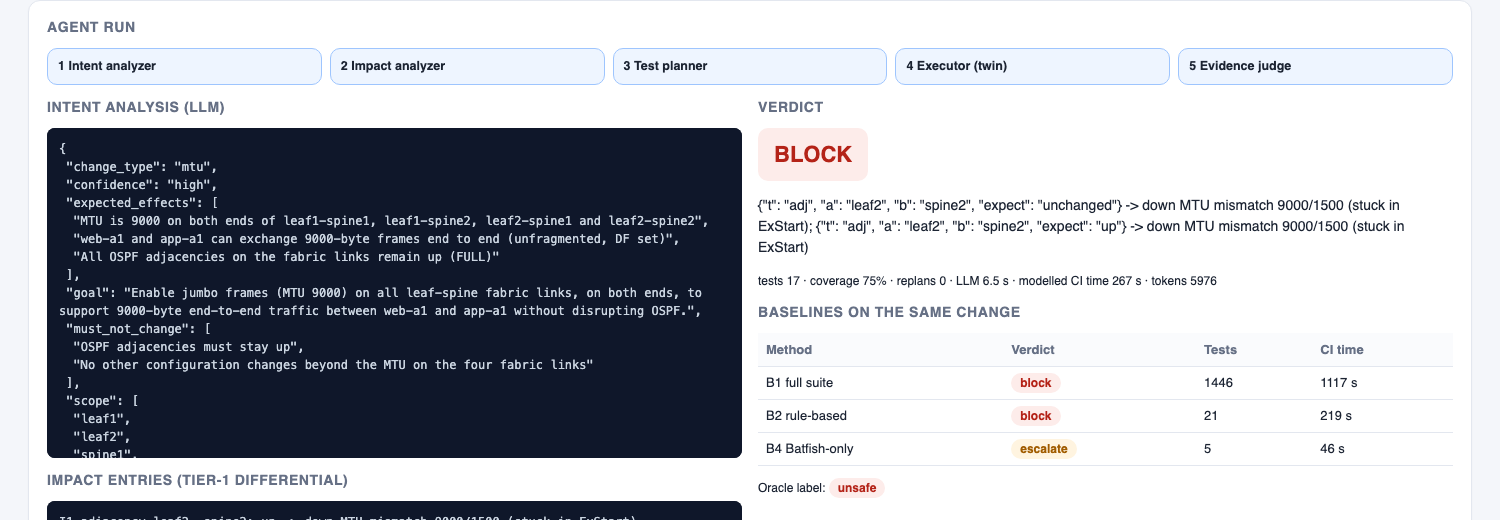
\includegraphics[width=0.7\textwidth]{figures/gui_case_block_top.png}
\caption{Prototype web interface validating a faulty jumbo-frame change (D-MTU-1-F, clear ticket): the impact analyzer finds the OSPF adjacency stuck in ExStart and the gate blocks with 17 tests, whereas B1 needs 1{,}446 tests.}\label{fig:gui}
\end{figure*}

\end{appendices}

\bibliography{references}

\end{document}
